%pdflatex
%!TEX TS-program = pdflatex
%!TEX encoding = UTF-8 Unicode
%
% PLANTILLA PARA UN TRABAJO DE FIN DE GRADO
% EN EL GRADO DE MATEMÁTICAS DE LA UNIVERSIDAD DE ZARAGOZA
%
% Mario Pérez Riera
% Área de Análisis Matemático, Universidad de Zaragoza
%
% Última modificación: 1 de agosto de 2021
%
% Escrito para pdfLaTeX
%
%
\documentclass[11pt]{book}

% Paquetes y fuentes
%---------------------------------------------------------------------------
\usepackage{geometry}               % define las dimensiones de la página
\geometry{
 a4paper, % Tamaño del papel
 centering, % Zona útil centrada
 margin = 25mm, % Márgenes en blanco: 25mm
% includehead, % Incluir la cabecera en el área del texto
% includefoot, % Incluir el pie en el área del texto
}

\usepackage[utf8]{inputenc}        % para usar el teclado normalmente
\usepackage[spanish]{babel}        % selecciona idioma
\usepackage[T1]{fontenc}           % gestión de fuentes con acentos
\usepackage{textcomp}
\usepackage{appendix}
\usepackage[utf8]{inputenc} % si no está ya
\usepackage[T1]{fontenc}
\usepackage{listings}

\usepackage{xcolor}

% Si alguno de estos paquetes no los vas a usar, mejor los quitas:
\usepackage{amssymb}               % para cargar las fuentes de la A.M.S.
\usepackage{amsmath}               % para usar letras griegas en negrita
\usepackage{amsthm}                % mejora los entornos tipo-teorema y proof
\usepackage{mathptmx}              % fuente Times
%\usepackage{lmodern}              % fuente Times
\usepackage{tikz}                  % para los dibujos
\usepackage{float} % Para usar [H]
\usetikzlibrary{babel}              % para evitar conflictos entre TikZ y babel
\addto\captionsspanish{\renewcommand{\tablename}{Tabla}}

% --- Configuración para Listings (Código fuente) ---
\definecolor{codegreen}{rgb}{0,0.6,0}
\definecolor{codegray}{rgb}{0.5,0.5,0.5}
\definecolor{codepurple}{rgb}{0.58,0,0.82}
\definecolor{backcolour}{rgb}{0.95,0.95,0.92}

% Estilo base común para todos los lenguajes
\lstdefinestyle{codestyle}{
    backgroundcolor=\color{backcolour},   
    commentstyle=\color{codegreen},
    keywordstyle=\color{magenta},
    numberstyle=\tiny\color{codegray},
    stringstyle=\color{codepurple},
    basicstyle=\ttfamily\footnotesize,
    breakatwhitespace=false,         
    breaklines=true,                 
    captionpos=b,                    
    keepspaces=true,                 
    numbers=left,                    
    numbersep=5pt,                  
    showspaces=false,                
    showstringspaces=false,
    showtabs=false,                  
    tabsize=2,
    frame=single,
    rulecolor=\color{black!30},
}

% Estilo para Python
\lstdefinestyle{pythonstyle}{
    style=codestyle,
    language=Python,
    keywordstyle=\color{blue},
    morekeywords={self, True, False, None} % Añadir palabras clave si es necesario
}

% Estilo para R
\lstdefinestyle{rstyle}{
    style=codestyle,
    language=R,
    keywordstyle=\color{purple},
    morekeywords={function, return, if, else, read.csv} % Añadir palabras clave si es necesario
}



%\usepackage{longtable}             % permite saltos de páginas en tablas largas

%------ Enlaces en el pdf
\usepackage{url}
\usepackage[linesnumbered,ruled,vlined]{algorithm2e}


\usepackage[pdftex, colorlinks=true, citecolor=cyan, linkcolor=black, 
urlcolor=black]{hyperref}

%------ Cabeceras y pies de página
\usepackage{titleps}

\newpagestyle{miestilo}{
   \sethead[\thepage][][\textsl{\chaptername\ \thechapter. \chaptertitle}]
   {\textsl{Técnicas de ML aplicadas a la estimación del VaR y otras medidas \ - \ Hugo Naudín López}}{}{\thepage}
   %\setfoot[][\textsl{\thesection. \sectiontitle}][]
   %{}{\textsl{\thesection. \sectiontitle}}{}
}


\newpagestyle{primeraparte}{
%-- Cabecera par y cabecera impar
\sethead[\thepage][][\textsl{\chaptertitle}]
{\textsl{Una plantilla para el TFG \ - \ Mario Pérez Riera}}{}{\thepage}
%-- Pie de página par y pie de página impar
%\setfoot[][\textsl{\thesection. \sectiontitle}][]
%{}{\textsl{\thesection. \sectiontitle}}{}
}

%------ \S 4.3, p. 93, de The LaTeX Companion 1a ed. (Figura 4.2) (Juan Luis)
\newcommand{\clearemptydoublepage}{\newpage{\pagestyle{empty}\cleardoublepage}}
\newcommand{\sectionmarkwithoutsections}[1]{\markright{#1}}


\makeindex

\theoremstyle{plain} % Entornos tipo teorema
\newtheorem{teorema}{Teorema}[chapter]
%\newtheorem{lema}[teorema]{Lema} % La misma numeración que 'teorema'
\newtheorem{proposition}{Proposición}
\newtheorem{definition}{Definición}
\theoremstyle{definition} % Entornos tipo definición
\newtheorem*{defin}{Definición} % El asterisco hace que no se numere
%\newtheorem{ejemplo}{Ejemplo}

%------ Conjuntos de números
\newcommand\N{\mathbb{N}}
\newcommand\Z{\mathbb{Z}}
\newcommand\R{\mathbb{R}}
\newcommand\C{\mathbb{C}}

%------ Funciones en español
\renewcommand{\spanishoperators}{Re}
%\renewcommand{\spanishoperators}{Re ctg arc\,ctg} % Define \Re, \ctg, \arctg
\renewcommand{\lstlistingname}{Listado}

%-------------
\begin{document}
%-------------
\frontmatter                     % Parte primera del texto
\pagestyle{primeraparte}    % Estilo de cabeceras para la parte primera del texto

%\pagenumbering{roman} % Incluido en \frontmatter

%--- PORTADA DEL TFG
\begin{titlepage}
\begin{center}

\null
\vfill

\Huge{\bfseries Técnicas de aprendizaje automático aplicadas a la estimación del Valor a Riesgo y otras medidas de riesgo financiero}

\vfill

\noindent
\begin{figure}[h]
\centering

\includegraphics[width=100mm]{ciencias.png}\\%

\includegraphics[width=100mm]{logoUZ.png}
\end{figure}

\vfill

\Huge{\bfseries Hugo Naudín López}\\%
\Huge{Trabajo de fin de grado de Matemáticas}\\%
\Huge{Universidad de Zaragoza}\\%

\vfill
\huge{Junio de 2025}
\end{center}
\end{titlepage}
%--- FIN DE LA PORTADA

\clearemptydoublepage

%\setcounter{page}{7} % Por si queremos imponer un número de página

%--- RESUMEN
\chapter{Summary}
Risk management has become a crucial aspect of financial institutions 
and corporations, especially in the wake of the 2008 financial crisis. In 
order to avoid the same mistakes that led to the crisis, new regulations 
were put in place, which required financial institutions to improve their risk
management practices and develop more accurate risk prediction models.\\

The meaning of risk measure was formally defined and the 
characteristics that these measures should satisfy were established.
Value at Risk (VaR) and Expected Shortfall (ES) are two widely 
used risk measures in this field. The main goal of these is 
to quantify the potential losses (or returns lower than expected) of 
an investment, which is essential for making informed 
decisions. \\

The VaR is a general risk measure related to the quantiles of the 
distribution of the returns of an investment. Let $G_t$ be the random variable 
that represents the returns of an investment at time $t$, the VaR at a 
confidence level $\alpha$ is defined as the value that satisfies the following 
equation:
\begin{align*}
   \mathbb{P}\{G_t \leq VaR_{\alpha, t}\} = 1-\alpha
\end{align*}
This means VaR represents the pessimistic scenario of the returns of an
investment, which is the maximum loss that can be expected with a certain 
confidence. On the other hand, the ES is the expected 
return given that the return is below the VaR, which is formally defined 
as:
\begin{align*}
   ES_{\alpha, t} = \mathbb{E}(G_t|G_t \leq VaR_{\alpha, t})
\end{align*}
The joint use of these two measures provides a more complete 
picture of the risk associated with an investment. \\

Because of the importance of these measures, the ways to estimate them 
have been studied and improved throughout the years, as the 
precision and accuracy of the estimates are crucial. Linear regression 
is a basic statistical method that allows us to estimate the relationship between variables based on observed data. However, this technique has limitations, as it assumes 
linear relationships and can struggle with complex, nonlinear patterns 
present in real-world financial data.\\

To overcome these limitations, more sophisticated methods, as machine 
learning techniques, have been explored throughout this work. These 
techniques are theoretically more capable of capturing more complex 
relationships in the data, which can lead to more accurate estimations. \\

Many ML techniques can be used, but, in this work, the focus will be on 
two of them: Boosting and Neural Networks. Boosting is an 
ensemble learning technique that combines the predictions of several
weak learners to create a strong learner. It is particularly effective for
regression tasks, as it can capture complex relationships in the data, which 
will be helpful for the issue at hand. On the other hand, Neural Networks are
a powerful class of models that can learn complex patterns in data.
They are particularly useful for high-dimensional data and can capture
nonlinear relationships, which can be beneficial for estimating risk measures.\\

This work provides a theoretical approach to the concepts of VaR and ES,
as well as the basis of estimation methods just mentioned. Finally, 
the performance of these methods will be compared in terms of their
accuracy and reliability in estimating the VaR and ES of a set of
financial assets. \\

In the first chapter, the concepts of risk and risk measures are introduced, 
along with their characteristics and the reason why they are important. After 
that, the VaR and ES are defined, along with their advantages and
disadvantages, also giving a general perspective on its use cases.\\

In the second chapter, the focus shifts to the models used to estimate 
these measures. Firstly, statistical basics are introduced, as the 
relationship between quantiles and expectiles and risk measures 
is the basis of the estimation methods. Then, we introduce the basic 
regression techniques, giving a theoretical overview. After that, 
the main theme centers on the machine learning techniques used to 
estimate the VaR and ES. \\

Finally, the third chapter presents a practical application of the 
methods presented. First, the aim is to determine the best 
method among all and then, a use case is presented, where the 
VaR and ES of a real state asset are estimated, which could help an investor decide whether the investment is profitable or not. \\

This work includes appendices where Regression Trees 
techniques, which are used in the Boosting method, the optimization 
techniques used to improve the performance of the estimation methods and 
the code used to implement the methods and the use case are explained.\\
%--- FIN DEL RESUMEN

\clearemptydoublepage

\tableofcontents

\clearemptydoublepage

%-------------
\mainmatter                      % Parte principal del texto
\pagestyle{miestilo}    % Estilo de cabeceras para la parte principal del texto

%--- CAPÍTULO 1 DEL TFG
\chapter{Introducción: el riesgo en las inversiones}
A la hora de invertir, el interés de las corporaciones financieras es maximizar 
el beneficio y minimizar las pérdidas. Para ello, las compañías utilizan 
herramientas entre las que se encuentra la gestión del riesgo. El riesgo 
es la incertidumbre sobre la evolución de un activo, e indica la posibilidad 
de que una inversión ofrezca un rendimiento distinto del esperado, por lo 
que la gestión y el control de este puede ayudar a minimizar las pérdidas y 
optimizar las ganancias.\\

Durante la década de los 80, la Comisión de Bolsa y Valores de los Estados 
Unidos (SEC) comenzó a divulgar cómo las empresas estaban expuestas a la 
volatilidad de los mercados financieros, introduciendo y dando gran 
importancia al concepto de riesgo en el sistema, debido a los acontecimientos 
vividos en aquel entonces (Lunes Negro en 1987 y la Crisis de Ahorros y 
Préstamos). Más adelante, a partir de la crisis financiera del año 2008 y el 
acuerdo de Basilea III~\cite{BIS}, las políticas del riesgo que podían correr los bancos 
a la hora de conceder créditos y realizar inversiones se endurecieron, lo que 
hizo que los modelos de predicción y gestión de riesgo se optimizaran y 
mejoraran de manera considerable.\\

Por otra parte, el uso de la inteligencia artificial (IA) y los algoritmos basados 
en el aprendizaje automático se han incrementado en los últimos años, llegando 
a introducirse también en el campo financiero y en la implementación de 
modelos alternativos a la hora de gestionar el riesgo. \\
\section{Medidas de riesgo y sus características}
Las medidas de riesgo son funciones que asignan a una posición financiera 
(representada por una variable aleatoria $X$ que representa las ganancias) un 
número real que cuantifica su nivel de riesgo. Existen varias clases de medidas 
de riesgo según las características que cumple. Sean $X$ e $Y$ dos variables 
aleatorias que representan las ganancias de dos posiciones financieras y 
sea $\lambda$ una medida de riesgo. De acuerdo a~\cite{FS08}, 
las principales características son las 
siguientes: 
\begin{enumerate}
   \item \textbf{Monotonía} Si $X \leq Y$ casi seguro, entonces $\lambda(X) \geq \lambda(Y)$.
   \item \textbf{Invarianza ante el efectivo} Sea $c \in \mathbb{R}$ una 
   cantidad de efectivo, entonces se cumple que $\lambda(X+c) = \lambda(X)- c$.
   \item \textbf{Convexidad} Sea $w \in [0,1]$ una proporción de inversión, entonces
   $\lambda(wX + (1-w)Y) \leq w\lambda(X) + (1-w)\lambda(Y)$.
   \item \textbf{Cuasiconvexidad} Sea $w \in [0,1]$ una proporción de inversión, entonces
   $\lambda(wX + (1-w)Y) \leq \max\{\lambda(X),\lambda(Y)\}$.
   \item \textbf{Homogeneidad} Sea $a > 0$ un escalar, entonces $\lambda(aX) = a\lambda(X)$.
   \item \textbf{Subaditividad}  $\lambda(X+Y) \leq \lambda(X) + \lambda(Y)$.
\end{enumerate}

\begin{definition}
   Una medida de riesgo $\lambda$ se dice general si cumple que es monótona 
   e invariante ante el efectivo.
\end{definition}
\begin{definition}
   Una medida de riesgo $\lambda$ se dice convexa si cumple que es general 
   y cumple la característica de convexidad. 
\end{definition}
\begin{definition}
   Una medida de riesgo $\lambda$ se dice coherente si cumple que es general, 
   homogénea, convexa y subaditiva.
\end{definition}

Se van a estudiar dos medidas ampliamente utilizadas en el ámbito financiero. 
Estas son el Valor a Riesgo (VaR) y el Expected Shortfall (ES). La primera es una 
medida de riesgo general, ya que no es subaditiva~\cite{FS08}, 
mientras que la segunda es una medida de riesgo coherente. Ambas
medidas se usan para cuantificar el riesgo en inversiones y su estimación 
es fundamental para la toma de decisiones financieras. \\

\section{Valor a Riesgo (VaR)}

Si bien el concepto del VaR existe desde mucho antes, la definición del término y 
su difusión se debió a la publicación de un manual de referencia 
de J.P: Morgan en los años 90 acerca de la medición de riesgos~\cite{RM96}, 
lo cual hizo que se popularizara rápidamente.\\

\begin{definition}
   Sea $G_t$ una variable aleatoria que representa las ganancias de una 
   inversión en un tiempo $t$. Sea $F$ la función de distribución de
   $G_t$ y $\alpha$ un nivel de confianza específico. Entonces, el
   Valor a Riesgo (VaR) de $G_t$ en el tiempo $t$ con un nivel de confianza
   $\alpha$ se define como el valor que cumple lo siguiente:
   \begin{align*}
         \mathbb{P}\{G_t \leq VaR_{\alpha, t}\} = 1-\alpha
   \end{align*}
   Paralelamente, se puede definir de las siguientes maneras:
   \begin{align*}
      VaR_{\alpha, t} &= inf\{x\in \mathbb{R}:F(x)\geq 1-\alpha\}= F^{-1}(1-\alpha)
   \end{align*}
\end{definition}


\subsection{Ventajas y desventajas del VaR}
La medida VaR tiene una gran utilidad a la hora de limitar el riesgo y 
controlar las potenciales pérdidas (o retornos inferiores a lo esperado) 
de una inversión, pero hay otros aspectos en los que esta medida no es 
completa.\\

Por una parte, es una medida muy simple e intuitiva. Su significado y lo que 
representa es fácilmente comprensible, lo que hace que su utilización esté 
muy extendida. Además, la comparabilidad de dos distribuciones se puede 
realizar fácilmente mediante esta medida, lo que puede resultar útil para 
evaluar diferentes carteras o estrategias de inversión en términos de su riesgo 
potencial. Por ejemplo, al comparar dos activos, el VaR permite identificar 
cuál de ellos tiene una mayor probabilidad de incurrir en pérdidas superiores 
a un cierto umbral en un horizonte de tiempo definido. Esto facilita la toma 
de decisiones por parte de gestores de riesgo e inversores. Finalmente, 
hay en ocasiones en las que interesa la estabilidad de las medidas de riesgo. 
A la hora de hallar el VaR de una distribución, cualquier cuantil inferior al 
$1-\alpha$ puede tener cualquier valor, pero el VaR no variará, ya que es 
independiente de estos valores, siempre y cuando sean menores.\\

Sin embargo, que el VaR no varíe aunque los cuantiles menores sí puede ser 
negativo desde otro punto de vista. Esto significaría que una mínima variación 
del nivel de confianza significaría una gran variación del VaR. Por tanto, esta 
medida estaría ocultando un riesgo mayor del que parece en un principio. \\

Esta desventaja hace del VaR una medida que, a pesar de su gran utilidad, 
presenta una notable incompletitud. Por ello, existen otras medidas que 
complementan esta primera, ofreciendo una extensión a la información del 
VaR, sobre todo, dando información del cuantil inferior. Entre estas 
variables se encuentra el Expected Shortfall (ES) o Valor a Riesgo
Condicional (CVaR). 

\section{Expected Shortfall (ES) o Valor a Riesgo Condicional (CVaR)}
El Expected Shortfall (ES) o Valor a Riesgo Condicional (CVar) son dos términos
relacionados con el mismo concepto. Para no sobrecargar la notación, se referirá a este 
concepto como ES de aquí en adelante. Su definición y explicación fueron 
presentadas por Carlos Acerbi y Dirk Tasche en 2002~\cite{AT02a} \cite{AT02b}.\\
\begin{definition}
   Sea $G_t$ una variable aleatoria que representa las ganancias de una 
   inversión en un tiempo $t$. Sea $\alpha$ un nivel de confianza específico. 
   Entonces, el ES de $G_t$ en el tiempo $t$ con un nivel 
   de confianza $\alpha$ se define como la esperanza condicional de
   $G_t$ dado que $G_t$ es menor o igual que el VaR en ese tiempo y nivel de
   confianza:
   \begin{align*}
      ES_{\alpha, t} = \mathbb{E}(G_t|G_t \leq VaR_{\alpha, t})\\
  \end{align*}
\end{definition}

El ES siempre será menor que el VaR, ya que 
el ES toma en cuenta los beneficios menores a él y, por lo tanto, refleja una 
evaluación más conservadora del riesgo. Si el VaR se considera como el 
valor máximo de pérdida en un nivel de confianza $\alpha$, el ES estima 
el valor promedio de las pérdidas cuando las pérdidas ya superan ese valor. 
Por lo tanto, el ES proporciona una medida más completa del riesgo 
asociado a eventos extremos.

\subsection{Ventajas y desventajas del ES}
La medida ES, al contrario del VaR, es una medida continua respecto a $\alpha$, 
es decir, cambios pequeños en el nivel de confianza no suponen cambios 
grandes en el ES. Si se toma un conjunto de inversiones $(X_i)_{i=1}^n$ y 
$(w_i)_{i=1}^n$ la proporción de cada inversión en nuestra cartera
($\sum_{i=1}^n w_i = 1$), entonces la medida ES en un tiempo $t$ con una 
confianza $\alpha$ es convexa~\cite{FS08} respecto a la  combinación de estas variables:
\begin{align*}
   ES_{\alpha, t}(w_1X_1+\dots w_nX_n) \leq w_1ES_{\alpha, t}(X_1)+\dots w_nES_{\alpha, t}(X_n)
\end{align*}
lo cual es coherente con la idea de la diversificación de activos para la 
reducción del riesgo, ya que el ES de la cartera nunca excede el promedio 
ponderado de los ES individuales\\

Por otro lado, esta medida es muy sensible a los errores de estimación. 
Normalmente, no hay muchos datos en los cuantiles bajos, por lo que es 
necesario plantear un modelo para obtener más observaciones. Existen casos en los 
que estos modelos son erráticos y las estimaciones en las colas pueden desviarse de 
la realidad.\\

Por tanto, la utilización y corrección de esta medida depende en gran parte 
de la corrección y confianza que se tenga en los datos. Sin embargo, 
la combinación de esta medida con el VaR ofrece una visión muy 
completa del riesgo en la inversión.

\section{Interés de las medidas de riesgo}
Las medidas de riesgo, como el Valor en Riesgo (VaR) y Expected Shortfall (ES), 
son herramientas fundamentales en la gestión de riesgos, ya que permiten 
cuantificar y gestionar la incertidumbre asociada a las pérdidas potenciales 
en diferentes contextos. Su utilidad varía dependiendo de si se aplican a 
carteras de valores o al ámbito corporativo.
\subsection{VaR y ES orientados a carteras de valores}
En el ámbito de la gestión de carteras de inversión~\cite{SSU}, el VaR y el ES son 
cruciales para entender y controlar la exposición al riesgo.\\

En el caso del VaR, estima la pérdida máxima de una cartera de valores 
en un horizonte temporal específico y con un nivel de confianza dado. 
Permite a los gestores de carteras evaluar riesgos acumulativos, 
identificando el impacto potencial de eventos de mercado extremos sobre 
la cartera, tomar decisiones informadas, comparando diferentes estrategias 
de inversión en función de su perfil de riesgo y cumplir requisitos 
regulatorios (normativas de Basilea).\\

El ES complementa al VaR al estimar la pérdida promedio en los casos en 
que esta exceda el VaR. Es especialmente útil porque ofrece una visión más 
completa y optimiza carteras.\\

Las dos medidas juntas son esenciales para medir y gestionar el riesgo de 
mercado, mejorar la asignación de activos y proteger a los inversores frente 
a pérdidas inesperadas.

\subsection{VaR y ES orientados a inversiones inmobiliarias}
La utilización de estas medidas de riesgo en las inversiones inmobiliarias 
se enfoca en la predicción del precio de los alquileres de los inmuebles. 
Dado el precio de una vivienda, el VaR y el ES permiten estimar escenarios negativos 
de precios a los que puede ser alquilado, permitiendo estimar 
si la inversión es suficientemente rentable.\\

Al mismo tiempo, el VaR y el ES se pueden utilizar para calcular una 
cota inferior del valor intrínseco de una vivienda dadas unas características
específicas, como la ubicación, el tamaño y las condiciones del mercado.
Esto permite a los inversores evaluar si el precio de compra de una propiedad
es razonable en relación con su valor potencial de alquiler y su riesgo asociado.\\


\subsection{VaR y ES orientados a corporaciones}
En el contexto corporativo~\cite{OBU17}, estas métricas ayudan a evaluar el riesgo 
financiero y operativo que enfrentan las empresas en sus actividades.\\

El VaR se utiliza para medir riesgos asociados a las fluctuaciones en tipos de 
cambio, tasas de interés o precios de materias primas y a la toma de 
decisiones estratégicas.\\

Por su parte, el ES proporciona una perspectiva más amplia, considerando 
las pérdidas extremas que pueden no ser capturadas por el VaR. Ofrece un 
análisis más detallado de los escenarios de mayor impacto financiero y 
permite a las empresas diseñar planes de mitigación y estrategias para 
afrontar eventos inesperados.\\

En el ámbito corporativo, estas medidas de riesgo facilitan la identificación 
de vulnerabilidades clave, la planificación financiera y la protección de los 
recursos de la empresa frente a incertidumbres del entorno operativo y del 
mercado.

\subsection{VaR y ES orientados a predicciones de impago en créditos}
Estas variables económicas también se emplean en la predicción de impago 
de créditos~\cite{KO17}, lo que ayuda a los bancos y entidades de préstamos en sus 
decisiones.
El VaR se utiliza para estimar la cantidad que con un nivel de confianza dado 
el cliente impagará, considerando factores como el historial crediticio, la 
situación financiera, las condiciones del mercado y determinadas 
características del cliente. \\

Por otra parte, el ES, al igual que en el caso de las carteras de valores, se 
utiliza para evaluar la pérdida promedio en los casos en que el cliente no 
pague, lo que da más información a la entidad acerca de la rentabilidad de 
dar el crédito.\\

Estas medidas permiten a las entidades evaluar el riesgo asociado a la 
concesión de créditos y ajustar sus políticas de préstamo en consecuencia.\\


\chapter{Modelos de riesgo}
%--- CAPÍTULO 2 DEL TFG
Con el objetivo de aproximar las medidas de riesgo anteriormente descritas, 
a lo largo de la historia se han ido desarrollando diferentes modelos que 
emplean técnicas distintas para ayudar a predecir el riesgo dadas distintas 
situaciones.
\section{Modelos tradicionales}
Los métodos tradicionales están fundamentados en la econometría y en 
métodos estadísticos. Sin embargo, algunos de estos enfoques pueden presentar 
limitaciones cuando se enfrentan a condiciones de mercado altamente 
volátiles o a eventos inesperados o se basan en suposiciones 
no siempre ciertas (distribuciones normales, independencia de errores, etc.). 
Sin embargo, existen otras técnicas que tienen una mayor robustez. 
\subsection{Regresión cuantil}
Para introducir los conceptos que se van a presentar, se toma $X$ una 
variable aleatoria continua con función de distribución  
$F: \mathbb{R} \to [0,1]$ y función de densidad $f_X$. Se fija un nivel 
$\alpha \in (0,1)$.
\begin{definition}
   El cuantil de orden $\alpha$ de la variable aleatoria $X$, denotado $c_\alpha(X)$, 
   se define como:
      \begin{align*}
         c_\alpha(X) := F^{-1}(\alpha) = \inf \{ x \in \mathbb{R} : F(x) \geq \alpha \}
      \end{align*}
   \end{definition}

La regresión cuantil \cite{K05} es un método estadístico que permite estimar la 
relación entre variables explicativas con los cuantiles de la distribución 
de la variable dependiente. A diferencia de la regresión lineal usual, 
que se centra en la media condicional, la regresión cuantil proporciona una 
visión más completa de la relación entre variables al considerar los cuantiles 
de la distribución, de donde se puede obtener una información mayor.\\

Para introducir la regresión cuantil, conviene partir de una formulación general 
de los modelos de regresión. Se considera un conjunto de variables 
explicativas $ \mathbf{X}_i = \{X_{i1}, X_{i2}, \dots, X_{ik} \}$ y una variable 
dependiente $Y_i$. La regresión lineal modela la esperanza condicionada 
de la variable dependiente en función de las variables explicativas mediante la 
utilización de los parámetros 
$\hat{\beta} = (\hat{\beta}_0, \hat{\beta}_1 \dots  , \hat{\beta}_k)$ de la siguiente 
manera:
\begin{align*}
    \hat{Y}_i= \mathbb{E}(Y_i | \mathbf{X_i}) = \hat{\beta}_0 + \hat{\beta}_1 X_{i1} + \hat{\beta}_2 X_{i2} + \cdots + \hat{\beta}_k X_{ik}
\end{align*}

 Los coeficientes $\hat{\beta}_j$ se denominan coeficientes de regresión 
y cuantifican la influencia de cada variable explicativa sobre la respuesta.
El objetivo de la regresión es estimar los parámetros $\hat{\beta}_j$ que mejor 
aproximen la relación entre $Y_i$ y $\mathbf{X_i}$. 

La regresión cuantil intenta modelar el cuantil $\alpha$ de la 
variable dependiente $Y_i$ dado un conjunto de variables explicativas 
$\mathbf{X_i}$, en vez de centrarse en la media. La forma general del modelo es:
\begin{align*}
    c_{\alpha}(Y_i|\mathbf{X}_i) = \dot{\beta}_0(\alpha)+ \dot{\beta}_1(\alpha)X_{i1}+ \dot{\beta}_2(\alpha)X_{i2}+\cdots +  \dot{\beta}_k(\alpha)X_{ik}
\end{align*}
donde $c_{\alpha}(Y_i|\mathbf{X}_i)$ es el cuantil $\alpha$ de la 
variable dependiente $Y_i$ dado el vector de variables explicativas 
$\mathbf{X}_i$. \\

Para hallar los parámetros $\dot{\beta}$, se utiliza una función de pérdida, la 
cual se debe intentar minimizar. En el caso de la regresión cuantil, la función 
de pérdida empleada es la función de pérdida cuantílica o pinball. 
\begin{definition}
La función de pérdida cuantílica de orden $\alpha \in (0,1)$, se define como:
   \begin{equation}
   \rho_\alpha(r) := r(\alpha - \mathbb{I}\{r < 0\}), \quad r \in \mathbb{R}.
   \label{eq:pinball}
   \end{equation}
\end{definition}

\begin{proposition}
El valor de $\theta \in \mathbb{R}$ que minimiza el valor esperado de la función 
de pérdida cuantílica es el cuantil de orden $\alpha$ de $X$, es decir:
   \begin{align*}
      \arg\min_{\theta \in \mathbb{R}} \mathbb{E}_X[\rho_\alpha(X - \theta)] = c_\alpha(X)
   \end{align*}
\end{proposition}

\begin{proof}
Se considera la función objetivo:
\begin{align*}
   g(\theta) := \mathbb{E}_X[\rho_\alpha(X - \theta)] = \int_{-\infty}^{\infty} (x - \theta)(\alpha - \mathbb{I}\{x < \theta\}) f_X(x) \, dx
\end{align*}
Bajo la hipótesis de que $f_X$ es continua, esta función es diferenciable en 
$\theta$, y se puede calcular su derivada teniendo en cuenta que los extremos 
de integración dependen de $\theta$:
\begin{align*}
   g'(\theta) &= \frac{d}{d\theta} \left[ \int_{-\infty}^{\theta} (x - \theta)(\alpha - 1) f_X(x) \, dx + \int_{\theta}^{\infty} (x - \theta)\alpha f_X(x) \, dx \right]
\end{align*}

Aplicando la regla de Leibniz:

\begin{align*}
   g'(\theta) &= (\alpha - 1) \left[ (x - \theta) f_X(x) \big|_{x = \theta} + \int_{-\infty}^{\theta} \frac{d}{d \theta}[(x - \theta)] f_X(x) \, dx \right] \\
   &\quad + \alpha \left[ (x - \theta) f_X(x) \big|_{x = \theta} + \int_{\theta}^{\infty} \frac{d}{d \theta}[(x - \theta)] f_X(x) \, dx \right] \\
   &= (\alpha - 1)(0 \cdot f_X(\theta)) - (\alpha - 1)\int_{-\infty}^{\theta} f_X(x) \, dx \\
   &\quad + \alpha (0 \cdot f_X(\theta)) - \alpha \int_{\theta}^{\infty} f_X(x) \, dx \\
   &= -(\alpha - 1) F(\theta) - \alpha (1 - F(\theta)) \\
   &= F(\theta) - \alpha
\end{align*}

Como se quiere hallar el mínimo, se iguala la derivada a 0:
\begin{align*}
   g'(\theta) = 0 \quad \Longleftrightarrow \quad F(\theta) = \alpha \quad \Longleftrightarrow \quad \theta = F^{-1}(\alpha).
\end{align*}

Por tanto, el valor que minimiza la pérdida esperada es el cuantil de orden 
$\alpha$ de $X$.
\end{proof}

La estimación del cuántil no es trivial y se utilizan varios algoritmos para 
hallar los coeficientes de regresión $\dot{\beta}$~\cite[p.~11]{MC20}. Estas 
técnicas serán también relevantes a la hora de estudiar la regresión expectil, 
cuya función de pérdida es asimétrica y cuadrática, la cual se presentará 
más adelante. \\

Una vez se estiman los coeficientes, se podrá hacer una predicción de los 
cuantiles de la variable dependiente $Y_i$ dado un conjunto de variables 
explicativas $\mathbf{X_i}$.\\

La utilidad de la regresión cuantil reside, entre otras, en la facilidad para 
el cálculo del VaR, ya que permite estimar beneficios extremadamente bajos 
(incluso negativos) y relacionarlos con otros factores como las tasas de interés,
los precios de las materias primas o las condiciones del mercado, todo ello 
sin depender de la media ni de supuestos de normalidad.


\subsection{Regresión expectil}
Además de los cuantiles, existe una medida estadística de gran utilidad 
para la estimación del riesgo llamada expectil~\cite{NP87}. Para introducir los conceptos que se van a presentar, se toma $X$ una 
variable aleatoria continua con función de distribución  
$F: \mathbb{R} \to [0,1]$ y función de densidad $f_X$. Se fija un nivel 
$\tau \in (0,1)$.
\begin{definition}
   El expectil de orden $\tau$ ($e_\tau$) de la variable 
   aleatoria $X$ es aquel valor que minimiza la función $\phi(X-e_\tau)$, donde:
   \begin{align*}
      \phi(r) = 
      \begin{cases}
            \tau \cdot  r^2 & \text{si } r > 0 \\
            (1 - \tau)r^2 & \text{si } r \leq 0
      \end{cases}
   \end{align*}
   Esta función se denomina función de pérdida expectílica de orden $\tau$.
\end{definition}


Los expectiles se pueden utilizar como una aproximación de los cuantiles, 
aunque no son exactamente lo mismo. Mientras que los cuantiles dividen la
masa de probabilidad en proporciones fijas, los expectiles ponderan las 
pérdidas de manera diferente, dando más peso a pérdidas extremas. 
Por tanto, la aproximación no es la manera correcta de usarlos. \\

La regresión expectil es un método estadístico útil para estimar variables 
relacionadas con la cola de una distribución como, por ejemplo, 
el Expected Shortfall (ES). 
Mientras que la regresión cuantil minimiza una función de pérdida absoluta 
asimétrica, la regresión expectil minimiza una función de pérdida cuadrática 
asimétrica.\\

\begin{definition}
   La función de pérdida expectil de orden $\tau \in (0, 1)$ se denota: 
   \begin{equation}
      \phi_{\tau}(r) = 
      \begin{cases}
            \tau \cdot  r^2 & \text{si } r > 0 \\
            (1 - \tau)r^2 & \text{si } r \leq 0
      \end{cases}
      \label{eq:expectil_loss_function}
   \end{equation}
\end{definition}

Dadas unas variables explicativas $\mathbf{X_i} = \{X_{i1}, X_{i2}, \dots, X_{ik}\}$ y 
una variable dependiente $Y_i$, la regresión expectil se define como:
\begin{align*}
    e_\tau(Y_i|\mathbf{X_i})= \bar{\beta}_{0}(\tau)+ \bar{\beta}_{1}(\tau)X_{i1}+ \bar{\beta}_{2}(\tau)X_{i2}+\cdots +  \bar{\beta}_{k}(\tau)X_{ik} = \bar{\beta}(\tau)  \mathbf{X_i}
\end{align*}
y dado un conjunto de datos $(Y_i, \mathbf{X_i})_{i=1}^n$, la estimación de los
coeficientes de regresión expectil $\bar{\beta}(\tau)$ se obtiene minimizando la
función de pérdida expectílica:
\begin{align*}
    \bar{\beta}(\tau) = argmin_{\beta}\sum_{i=1}^n\phi_{\tau}(Y_i-e_{\tau}(Y_i|\mathbf{X}_i))
\end{align*}

\begin{proposition}
   Dado $ES_\alpha$ el Expected Shortfall de una variable aleatoria $X$ de orden 
   $\alpha$, se puede expresar en funcion de un expectil de orden $\tau$ que 
   cumple que su valor es igual al $VaR_{\alpha}$
   ($e_\tau = VaR_{\alpha} \Longleftrightarrow P(X \leq e_\tau) =1-\alpha$).
   
\end{proposition}
\begin{proof}
   Se puede definir la función de pérdida expectílica como: 
   \begin{align*}
       \phi_{\tau}(X - e_\tau) &= \tau(X - e_\tau)^2 I(X > e_\tau) + (1 - \tau)(X - e_\tau)^2 I(X \leq e_\tau) \\
        &= (\tau I(X > e_\tau) + (1 - \tau)I(X \leq e_\tau))(X - e_\tau)^2 \\
   \end{align*}
   Se va a desarrollar y obtener propiedades del expectil. Para ello, 
   se va a tomar un parámetro $\theta$ en lugar del expectil y a ver cual es  el 
   valor de $\theta$ que minimiza la esperanza de la función.
   \begin{align*}
      g_{\tau, \theta}(X) = (\tau I(X > \theta) + (1 - \tau)I(X \leq \theta))(X - \theta)^2 
   \end{align*}
   Se calcula su esperanza:
   \begin{align*}
      E_{X}(g_{\tau, \theta}(X)) &= E_{X}((\tau I(X > \theta) + (1 - \tau)I(X \leq \theta))(X - \theta)^2) = \\
      &= \int_{-\infty}^{\infty}(\tau I(x > \theta) + (1 - \tau)I(x \leq \theta))(x - \theta)^2 f_X(x)dx = \\
      &= \int_{-\infty}^{\theta}((1 - \tau)(x - \theta)^2 f_X(x)dx + \int_{\theta}^{\infty}(\tau (x - \theta)^2 f_X(x)dx = \\
      &= (1 - \tau)\int_{-\infty}^{\theta}(x - \theta)^2 f_X(x)dx + \tau \int_{\theta}^{\infty}(x - \theta)^2 f_X(x)dx
   \end{align*}
   Se deriva con respecto a $\theta$ y se iguala a $0$:
   \begin{align*}
      \frac{d}{d\theta}E_{X}(g_{\tau, \theta}(X)) &= (1 - \tau)\int_{-\infty}^{\theta}2(x - \theta)f_X(x)dx + (1 - \tau)(\theta - \theta)^2 f_X(\theta) + \\
      &\quad + \tau\int_{\theta}^{\infty}2(x - \theta)f_X(x)dx + \tau(\theta - \theta)^2 f_X(\theta) = \\
      &= (1 - \tau)\int_{-\infty}^{\theta}2(x - \theta)f_X(x)dx + 2\tau\int_{\theta}^{\infty}(x - \theta)f_X(x)dx = \\
      &= 2((1-\tau)E_{X}((X-\theta)\cdot 1_{X\leq \theta}) + \tau E_{X}((X-\theta)\cdot 1_{X >\theta})) = 0
   \end{align*} 
   Por tanto, simplificando, se tiene que:
   \begin{align*}
      E_{X}((X-\theta)\cdot 1_{X > \theta}) = -\frac{1-\tau}{\tau}E_{X}((X-\theta)\cdot 1_{X \leq \theta})
   \end{align*}
   y sustituyendo $\theta$ por $e_\tau$, se tiene que:
   \begin{align*}
      E_{X}((X-e_\tau)\cdot 1_{X> e_\tau}) = -\frac{1-\tau}{\tau}E_{X}((X-e_\tau)\cdot 1_{X\leq e_\tau})
   \end{align*}
   Se denota $A = E_{X}((X-e_\tau)\cdot 1_{X> e_\tau})$ y $B = E_{X}((X-e_\tau)\cdot 1_{X\leq e_\tau})$, por lo que:
   \begin{align*}
      A = -\frac{1-\tau}{\tau}B
   \end{align*}
   Sabiendo que $1-\alpha = P(X \leq e_\tau)$, por lo que:
   \begin{align*}
      E_{X}((X-e_\tau)\cdot 1_{X \leq e_\tau}) &= \int_{-\infty}^{e_\tau}(x-e_\tau)f_X(x)dx = \int_{-\infty}^{e_\tau}xf_X(x)dx - e_\tau \int_{-\infty}^{e_\tau}f_X(x)dx = \\
      &= \frac{1-\alpha}{1-\alpha}\int_{-\infty}^{e_\tau}xf_X(x)dx - e_\tau (1-\alpha) = (1-\alpha) (ES_\alpha - e_\tau)
   \end{align*}
   Por tanto, despejando $ES_\alpha$:
   \begin{align*}
      ES_\alpha &= \frac{1}{1-\alpha}E_{X}((X-e_\tau)\cdot 1_{X \leq e_\tau}) + e_\tau
   \end{align*}
   Se desea una expresión más sencilla. Se suma A y B, calculados anteriormente:
   \begin{align*}
      A + B &= E_{X}((X-e_\tau)\cdot 1_{X > e_\tau}) + E_{X}((X-e_\tau)\cdot 1_{X\leq e_\tau}) = \\
      &= E_{X}(X-e_\tau) = E_{X}(X) - e_\tau
   \end{align*}
   Al mismo tiempo, 
   \begin{align*}
      A+B = -\frac{1-\tau}{\tau}B + B = \left(1 - \frac{1-\tau}{\tau}\right)B = \frac{2\tau-1}{\tau}B 
   \end{align*}
   Por tanto, sustituyendo en la expresión anterior:
   \begin{align*}
      ES_\alpha &= \frac{1}{1-\alpha}B + e_\tau = \frac{1}{1-\alpha}E_{X}((X-e_\tau)\cdot 1_{X \leq e_\tau}) + e_\tau = \\
      &= \frac{\tau}{(1-\alpha) \cdot (2\tau-1)} (E_X(X)-e_\tau)+e_\tau \\
   \end{align*}

\end{proof}
Por tanto, se utilizará la estimación de los expectiles para estimar el orden $\tau$
para el que el expectil $e_\tau$ coincide con el VaR 
($P(X \leq e_\tau) = 1-\alpha \implies e_\tau = Var_\alpha$). Una vez se tenga 
el expectil, se podrá estimar el Expected Shortfall (ES)~\cite{Taylor08}.

\section{Modelos basados en Machine Learning}
Conforme al avance de la tecnología, se han ido desarrollando nuevos métodos de 
estimación del riesgo, algunos basados en el aprendizaje máquina, que se ha desarrollado 
en los últimos años exponencialmente. Los métodos basados en Machine Learning (ML) 
son modelos de muchas dimensiones que se combinan con métodos de “regularización” y 
de reducción del sobreajuste, junto con algoritmos eficientes de búsqueda.\\

La base de los modelos de ML es parecida a la de los modelos econométricos, ya que están 
basados en métodos estadísticos. Sin embargo, existen diferencias entre los modelos que 
los vuelven muy diferentes.\\

Mientras que los modelos econométricos se centran en la inferencia causal y la 
interpretación de relaciones económicas, los modelos de ML se enfocan en la predicción 
y precisión del ajuste. Además, los modelos de ML no se basan en supuestos como la 
normalidad o la independencia, al contrario que muchos métodos econométricos, lo que 
los hace más fielmente aplicables a distintas situaciones. \\

Previo a la utilización de estos métodos, es necesario “entrenarlos”, es decir, ajustar los 
parámetros del modelo a los datos. Para ello, se dividen los datos en dos conjuntos: el 
conjunto de entrenamiento y el conjunto de prueba. El conjunto de entrenamiento se 
utiliza para ajustar el modelo, mientras que el conjunto de prueba se utiliza para evaluar 
su rendimiento. Una vez se entrena el modelo, se podrá aplicar sobre otros datos, 
obteniendo predicciones sobre el riesgo asociado a los eventos.\\

Se van a presentar a continuación modelos utilizados para la estimación de cuantiles y 
expectiles~\cite{HTF17}, que posteriormente se utilizarán en un caso práctico.

\subsection{Redes Neuronales}
Las redes neuronales funcionan como cerebros humanos, en los que se encuentran 
neuronas conectadas entre si. Están formadas por varios conjuntos de neuronas, llamados capas.  Hay tres tipos de capas, llamadas la capas de entrada, ocultas y de salida. 
Para entrenar a la red neuronal, se introducen los datos por la capa de entrada. A partir de 
ahí, la información se transporta por las capas ocultas mediante funciones predeterminadas 
y pesos que determinan la influencia entre neuronas interconectadas. Este proceso se 
repite hasta que la información llega a la capa de salida. El proceso de razonamiento 
interno funciona como una caja negra y no se puede identificar realmente las relaciones 
entre la entrada y la salida. \\

Para hacer una explicación completa pero sencilla, se tomará una red neuronal con 
una sola capa oculta totalmente conectada. Las entradas 
$ \mathbf{X}= \{X_{1}, X_{2}, \dots, X_{n} \}$  son 
transformadas mediante pesos y una función llamada función de activación y transportadas 
a la siguiente neurona, la cual está en la capa oculta. Acto seguido, se repetirá el proceso 
entre la capa oculta y la capa de salida pero utilizando $Z_j \; j= 1, 2, \dots, M_1$ como 
entradas.

\begin{figure}[h]
    \centering
    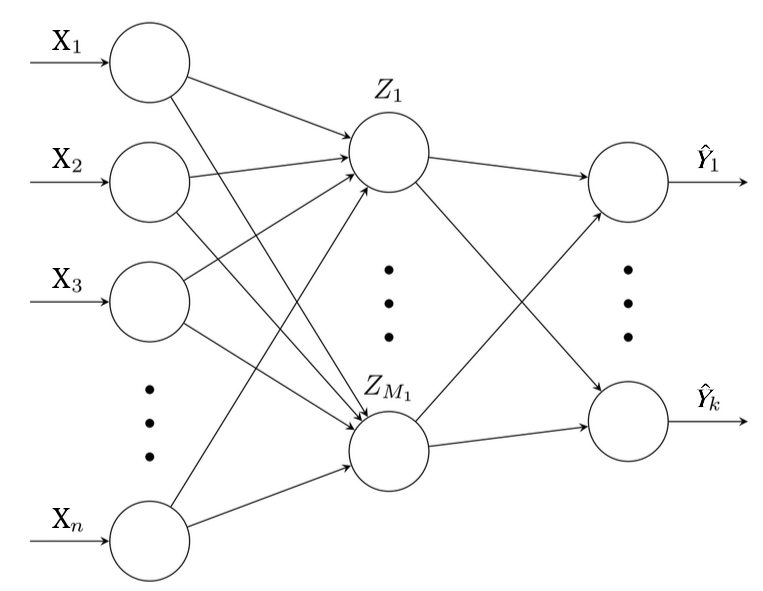
\includegraphics[width=0.5\textwidth]{picture1.jpg} 
    \caption{Esquema de una red neuronal artificial con una capa oculta.}
    \label{fig:miImagen} 
\end{figure}

Para cada neurona de la capa oculta, se transforman todos los valores de las neuronas 
de la capa de entrada de la siguiente manera:
\begin{align*}
    a_j^{(1)} &= \sum_{i=1}^n w_{j,i}^{(1)}X_i+b_{j}^{(1)}\\
    Z_j^{(1)} &= \sigma(a_j^{(1)})\:, j = 1, 2, \dots M_1
\end{align*}
con $\sigma$ la función de activación y $w_{j,i}$ los pesos asociados a cada neurona, 
además de un peso de la propia neurona receptora, llamada sesgo $b_{j}$. En caso de 
haber más  capas ocultas se repetiría este proceso:
\begin{align*}
    Z_j^{(m)} = \sigma\left(\sum_{i = 1}^{M_{(m-1)}}w_{j,i}^{(m)}Z_i^{(m-1)}+b_{j}^{(m)}\right)
\end{align*}
En el caso de la figura~\ref{fig:miImagen}, al solamente tener una capa oculta, la salida de la red 
neuronal será:
\begin{align*}
\hat{Y}_k = \sigma\left(\sum_{i=1}^{M_1} w_{k,i}^{(2)}Z_i^{(1)}+b_{k}^{(2)}\right)
\end{align*}
Tras obtener los resultados de la primera evaluación, se actualizan los pesos de la 
red intentando minimizar la siguiente función:
\begin{align*}
   \mathcal{L}(\mathbf{Y}, \mathbf{\hat{Y}}) = \sum_{i=1}^n \rho(Y_i - \hat{Y}_i)
\end{align*}
Siendo $\hat{Y}_i$ el valor esperado. Es decir, se intentan modificar los pesos de manera que 
la predicción sea lo más parecida al valor que se busca. Se modificará la función $\rho$ 
en función de cuál sea el objetivo de cálculo de la red. \\

En cuanto a las funciones de activación, la más utilizada e implementada en la mayoría 
de métodos es la función ReLu:
\begin{align*}
      \sigma(x) = 
      \begin{cases}
         x & \text{si } x > 0 \\
         0 & \text{si } x \leq 0
      \end{cases} = \max(0, x)
\end{align*}

Una de sus principales ventajas es su simplicidad computacional y su capacidad para 
evitar el problema del gradiente desvanecido en regiones positivas, lo que mejora 
significativamente la eficiencia del entrenamiento mediante el método de descenso por 
gradiente. Además, su derivada es muy simple, lo que  permite una propagación del 
gradiente más estable en comparación con funciones como la sigmoide. \\


Para ajustar los pesos, se utilizará el algoritmo de retropropagación (backpropagation), que 
se basa en el cálculo del gradiente de la función de pérdida con respecto a los pesos.
Sin embargo, en lugar de utilizar el método del gradiente descendente clásico, cuyo uso es sencillo 
y fácil de comprender, se empleará el algoritmo \textit{Adam} (Adaptive Moment Estimation)~\cite{KB14}, 
que utiliza estimaciones adaptativas de la media y la varianza del gradiente para actualizar los 
parámetros de manera más eficiente.


Dado el gradiente de la función de pérdida con respecto a los pesos de la capa $l$, que se denota 
por $g^{(l)} = \frac{\partial \mathcal{L}}{\partial \theta}= -\sum_{i=1}^n \rho'\left(Y_i - \hat{Y}_i\right) \cdot \frac{\partial \hat{Y}_i}{\partial \theta}$, 
Adam calcula una estimación del primer momento (media) y  del segundo momento  (varianza) del 
gradiente mediante las siguientes ecuaciones:
\begin{align*}
   m^{(l)} &\gets \beta_1 m^{(l)} + (1 - \beta_1) g^{(l)} \\
   v^{(l)} &\gets \beta_2 v^{(l)} + (1 - \beta_2) (g^{(l)})^2\\
   m_b^{(l)} &\gets \beta_1 m_b^{(l)} + (1 - \beta_1) g_b^{(l)} \\
v_b^{(l)} &\gets \beta_2 v_b^{(l)} + (1 - \beta_2) (g_b^{(l)})^2 
\end{align*}
A continuación, se realiza una corrección del sesgo de estas estimaciones, importante en las 
primeras iteraciones:
\begin{align*}
   \hat{m}^{(l)} &= \frac{m^{(l)}}{1 - (\beta_1)^t} \quad \hat{v}^{(l)} = \frac{v^{(l)}}{1 - (\beta_2)^t}\\
   \hat{m}_b^{(l)} &= \frac{m_b^{(l)}}{1 - (\beta_1)^t} \quad \hat{v}_b^{(l)} = \frac{v_b^{(l)}}{1 - (\beta_2)^t}
\end{align*}
Finalmente, se actualizan los pesos y el sesgo
\begin{align*}
   w^{(l)} \gets w^{(l)} - \zeta \cdot \frac{\hat{m}^{(l)}}{\sqrt{\hat{v}^{(l)}} + \epsilon}\\
   b^{(l)} \gets b^{(l)} - \zeta \cdot \frac{\hat{m}_b^{(l)}}{\sqrt{\hat{v}_b^{(l)}} + \epsilon}
\end{align*}
donde $\zeta$ es la tasa de aprendizaje, $\beta_1$ y $\beta_2$ son los coeficientes de
decaimiento para los momentos (típicamente 0.9 y 0.999), $\epsilon$ es un pequeño valor positivo
para evitar divisiones entre 0 y $t$ es la iteración actual.\\

Se supone, por tanto, que se tienen $m$ datos disponibles 
$(\mathbf{X_1}, Y_1), (\mathbf{X_2}, Y_2), \dots, (\mathbf{X_m}, Y_m)$, donde $\mathbf{X_i}$ 
son las variables explicativas y $Y_i$ las variable dependientes. El algoritmo será:\\

\begin{algorithm}[H]
   \caption{Red neuronal }
   \SetKwInOut{Input}{Entrada}
   \SetKwInOut{Output}{Salida}

   Inicializar aleatoriamente los pesos $w^{(l)}$, sesgos $b^{(l)}$, y momentos $m^{(l)}, v^{(l)}, m_b^{(l)}, v_b^{(l)}$ para $l = 1, \dots, L$\;
   $t \gets 0$\;

   \tcp*[h]{Bucle de entrenamiento}\;
   \For{epoch = 1 \KwTo T}{
       \For{$i = 1$ \KwTo $m$}{
           $t \gets t + 1$\;
           
           \tcp*[l]{1. Propagación hacia adelante}
           $Z^{(0)} \gets \mathbf{X}_i$\;
           \For{$l = 1$ \KwTo $L$}{
               $a^{(l)} \gets w^{(l)} Z^{(l-1)} + b^{(l)}$\;
               $Z^{(l)} \gets \sigma^{(l)}(a^{(l)})$\;
           }
           $\hat{\mathbf{Y}}_i \gets Z^{(L)}$\;

           \tcp*[l]{2. Retropropagación (Cálculo de gradientes)}
           $\delta^{(L)} \gets \frac{\partial \mathcal{L}}{\partial \hat{y}_i} \cdot \sigma^{(L)'}(a^{(L)})$\;
           $g^{(L)} \gets \delta^{(L)} (Z^{(L-1)})^\top$; \quad $g_b^{(L)} \gets \delta^{(L)}$\;
           \For{$l = L-1$ \KwTo $1$}{
               $\delta^{(l)} \gets ((w^{(l+1)})^\top \delta^{(l+1)}) \circ \sigma^{(l)'}(a^{(l)})$\;
               $g^{(l)} \gets \delta^{(l)} (Z^{(l-1)})^{\top}$; \quad $g_b^{(l)} \gets \delta^{(l)}$\;
           }

           \tcp*[l]{3. Actualización de parámetros (Optimizador Adam)}
           \For{$l = 1$ \KwTo $L$}{
               \tcp*[l]{Actualizar momentos}
               $m^{(l)} \gets \beta_1 m^{(l)} + (1 - \beta_1) g^{(l)}$; \quad $m_b^{(l)} \gets \beta_1 m_b^{(l)} + (1 - \beta_1) g_b^{(l)}$\;
               $v^{(l)} \gets \beta_2 v^{(l)} + (1 - \beta_2) (g^{(l)})^2$; \quad $v_b^{(l)} \gets \beta_2 v_b^{(l)} + (1 - \beta_2) (g_b^{(l)})^2$\;
               
               \tcp*[l]{Corregir sesgos de los momentos}
               $\hat{m}^{(l)} \gets \frac{m^{(l)}}{1 - \beta_1^t}$; \quad $\hat{m}_b^{(l)} \gets \frac{m_b^{(l)}}{1 - \beta_1^t}$\;
               $\hat{v}^{(l)} \gets \frac{v^{(l)}}{1 - \beta_2^t}$; \quad $\hat{v}_b^{(l)} \gets \frac{v_b^{(l)}}{1 - \beta_2^t}$\;
               
               \tcp*[l]{Actualizar parámetros}
               $w^{(l)} \gets w^{(l)} - \zeta \frac{\hat{m}^{(l)}}{\sqrt{\hat{v}^{(l)}} + \epsilon}$\;
               $b^{(l)} \gets b^{(l)} - \zeta \frac{\hat{m}_b^{(l)}}{\sqrt{\hat{v}_b^{(l)}} + \epsilon}$\;
           }
       }
   }
\end{algorithm}
\hfill

Las redes neuronales tienen una gran capacidad de aprendizaje y alta precisión en 
tareas complejas. Estas son las características que hacen que su utilización esté muy 
extendida en modelos predictivos.\\

\subsection{Algoritmos de Boosting}
Los algoritmos de boosting~\cite{SF12} son una técnica de aprendizaje 
automático que se basa en la existencia de algoritmos débiles que, dados 
ejemplos de entrenamiento etiquetados, produce unos predictores débiles que, 
después, se combinan produciendo un predictor fuerte de alta precisión.\\

El objetivo es generar estos predictores de forma iterativa. En cada iteración, el predictor 
débil intenta corregir los errores del predictor anterior. Para ello, se modifica la importancia 
de cada dato dentro de la muestra para que cada clasificador débil se ''especialice'' en 
los datos cuya predicción ha sido errada por el anterior. Para predecir correctamente, 
el predictor débil trata de minimizar una función de pérdida, que se definirá dependiendo 
del objetivo del algoritmo.\\

Para ajustar el modelo, se debe entrenar, al igual que ocurre con las redes 
neuronales. Por tanto, para la explicación del modelo, se toman 
$(\mathbf{X_1}, Y_1), (\mathbf{X_2}, Y_2), \dots, (\mathbf{X_m}, Y_m)$, 
siendo $\mathbf{X_i}$ 
variables explicativas y $\mathbf{Y}_i$ las variables dependientes explicadas.
Se define $\mathbf{X} = \{\mathbf{X_1}, \mathbf{X_2}, \dots, \mathbf{X_m}\}$.\\

Asociando al predictor débil la función $g: \mathbb{R}^n \to \mathbb{R}$, la función de 
pérdida que tratará de minimizar será:
\begin{align*}
   \mathcal{L}(\mathbf{X}, \mathbf{Y}, g) = \sum_{i=1}^m \rho(Y_i - g(\mathbf{X}_i))
\end{align*}

Para estimar cuantiles se utilizará la función de pérdida 
cuantil o \textit{pinball loss}~\eqref{eq:pinball} y para calcular expectiles se usará la función de pérdida 
expectil~\eqref{eq:expectil_loss_function}.\\

Los predictores débiles que se utilizarán serán árboles de regresión, que son 
estructuras jerárquicas que dividen el espacio de las variables explicativas con el fin 
de minimizar el error de predicción en cada hoja. Los árboles utilizados en boosting son 
poco profundos, a menudo con una profundidad limitada, lo que los convierte en 
predictores débiles pero complementarios entre sí. Una descripción más detallada 
de los árboles de regresión se pueden encontrar en el \nameref{ap:arboles}.\\

Para la optimización de los predictores se utilizará el gradiente descendente. 
En lugar de ajustar directamente parámetros numéricos, se busca en cada 
iteración una función (el predictor débil) que apunte en la dirección del gradiente negativo de la función de pérdida.\\

Dado $f_{m-1}(x)$ el predictor fuerte en una iteración dada, se calcula el gradiente negativo 
de la pérdida con respecto a las predicciones.:
\begin{align*}
   \mathbf{u}_{i,m} = -\left.\frac{\partial \mathcal{L}(\mathbf{X}, \mathbf{Y}, f)}{\partial f(\mathbf{X}_i)}\right|_{f = f_{m-1}}
\end{align*}
Estos valores representan la dirección en la que debe moverse para minimizar la 
función de pérdida. El predictor débil $g_m(x)$ se ajusta entonces para aproximar 
estos residuos, y se actualiza el modelo sumando la nueva función escalada por un factor de aprendizaje $\eta$:
\begin{align*}
   f_m(x) = f_{m-1}(x) + \eta \cdot g_m(x)
\end{align*}

Cuanto más pequeña sea la tasa de aprendizaje $\eta$, más lento será el proceso, pero 
también más estable y menos propenso al sobreajuste. \\

El algoritmo de boosting es teóricamente ideal para afrontar el problema ya que 
$\mathbf{X_i}$ es una variable multidimensional y el problema puede tornarse complejo. 
La eficiencia y precisión de los algoritmos de boosting los hacen muy útiles en la 
estimación de cuantiles y expectiles.\\





\begin{algorithm}[H]
   \caption{Boosting para cuantiles y expectiles}
   
   Inicializar $f_0(x) \gets 0$ o $f_0(x) \gets \bar{y}$ (la media de los valores $y_i$)\;
   
   \For{$m = 1$ \KwTo $M$}{
       \For{$i = 1$ \KwTo $n$}{
           $u_{i,m} \gets -\rho'_\tau(y_i - f_{m-1}(x_i))$\;
       }
   
       \tcp*[l]{Ajustar un predictor débil $g_m(x)$ a los pares $(x_i, u_{i,m})$}
         $\{(x_i, u_{i,m}) \}_{i=1}^n \longrightarrow g_m(x)$\;
       $f_m(x) \gets f_{m-1}(x) + \eta \cdot g_m(x)$\;
   }
   \end{algorithm}
   


\chapter{Aplicaciones de modelos a inversiones inmobiliarias}

En este capítulo se va a presentar una aplicación de los modelos presentados en 
el capítulo anterior a un caso de inversión inmobiliaria. El objetivo va a ser la 
predicción de medidas de riesgo asociadas a inversiones inmobiliarias, modelando 
la mínima rentabilidad esperada de la inversión. \\

Un tipo de inversión inmobiliaria es la compra de inmuebles para su 
posterior alquiler. Siendo este el caso, el comprador debe estimar 
si merece la pena el precio de compra del inmueble, teniendo en 
cuenta los gastos asociados a la compra y, más importante, los ingresos 
esperados de ese alquiler. A la hora de acometer una inversión, se 
debe fijar un retorno mínimo anual esperado, al cual se referirá como 
rentabilidad mínima esperada, que se denotará $r_{min}$. En términos teóricos, 
se puede identificar el VaR con la renta mínima esperada, la cual 
se utilizará para hallar después $r_{min}$ y ayudará a decidir si 
una inversión es rentable o no. \\

Por otro lado, también es interesante estimar cuál sería la rentabilidad 
esperada en caso de ser menor que $r_{min}$, ya que ayudará a decidir 
si, pese a no alcanzar la rentabilidad mínima esperada, merece la pena asumir dicho riesgo. \\

Por tanto, el objetivo de este capítulo es la estimación de la renta
mínima esperada y la rentabilidad esperada en caso de ser menor 
que la mínima esperada con un nivel de confianza dado mediante los modelos presentados, utilizando datos 
de viviendas en la Comunidad de Madrid~\cite{ID25} mediante 
web scraping. Se han tomado 
todos los anuncios (aproximadamente 15000) de dicha web de viviendas para obtener una muestra 
relativamente grande que ayude a una más correcta estimación de los 
modelos. \\

Las variables utilizadas para su estimación han sido escogidas en base
a su relevancia teórica y su disponibilidad en los anuncios de Idealista y 
son las siguientes: 
\begin{itemize}
   \item \textbf{Precio de la vivienda:} Alquiler mensual al que se oferta
   \item \textbf{Superficie:} Tamaño de la vivienda en metros cuadrados
   \item \textbf{Número de habitaciones:} Número de habitaciones de la vivienda
   \item \textbf{Número de baños:} Número de baños de la vivienda
   \item \textbf{Planta:} Planta en la que se encuentra la vivienda (se considera que los bajos y entreplantas corresponden a la planta 0)
   \item \textbf{Latitud:} Coordenada geográfica norte-sur de la vivienda
   \item \textbf{Longitud:} Coordenada geográfica este-oeste de la vivienda
   \item \textbf{Ascensor:} Si la vivienda dispone de ascensor o no
   \item \textbf{Obra nueva:} Si la vivienda es de obra nueva o no
   \item \textbf{Piscina:} Si la vivienda dispone de piscina o no
   \item \textbf{Terraza:} Si la vivienda dispone de terraza o no
   \item \textbf{Garaje:} Si la vivienda dispone de garaje o no
   \item \textbf{Garaje incluido en el precio:} Si el garaje está incluido 
   en el precio del alquiler
   \item \textbf{Aire acondicionado:} Si la vivienda dispone de aire acondicionado o no
   \item \textbf{Trastero:} Si la vivienda dispone de trastero o no
   \item \textbf{Jardín:} Si la vivienda dispone de jardín o no
   \item  \textbf{Disponibilidad de planta:} Si la información acerca de la 
   planta en la que está la vivienda está disponible o no.
\end{itemize}

Una variable que se ha querido incluir pero no ha sido posible ha sido la 
fecha de construcción de la vivienda, que es esperable que influya con 
cierta importancia en el valor de alquiler de la vivienda. Sin embargo, 
dicho dato no está disponible en los anuncios de la web, por lo que se ha 
tenido que prescindir de él. \\

Al observar los datos, se ve que existen valores atípicos en el precio de
alquiler de las viviendas, que pueden influir negativamente en la estimación de 
los modelos. Por ello, se realizará en primer lugar un modelado con los 
datos originales y posteriormente se eliminarán los valores atípicos. Los valores atípicos se han identificado siguiendo un criterio conservador, tomando todos los datos por encima de 
$q_{0.75} + 1.5 * (q_{0.75} - q_{0.25})$, utilizando el criterio de rango intercuartílico
 (IQR).\\ 

Se va a entrenar a los modelos cuantílicos y se compararán los resultados obtenidos con la regresión cuantil y 
los modelos basados en machine learning. En primer lugar se separan 
los datos en dos conjuntos, uno de entrenamiento y otro de prueba, de 
forma aleatoria, tomando el 75\% de los datos para el entrenamiento y 
el 25\% restante para la prueba.

 \begin{table}[h!]
   \centering
   \begin{tabular}{|l|c|}
      \hline
      \textbf{Modelo} & \textbf{VaR Score (Pérdida Pinball)} \\
      \hline
      Regresión Cuantílica (QR) & 59,70 \\
      Red Neuronal Cuantílica (QNN) & 43,61 \\
      Boosting Cuantílico (QBR) & 39,87 \\
      \hline
   \end{tabular}
   \caption{Evaluación de los modelos de estimación del VaR ($\alpha=0.95$) en el conjunto de prueba.}
   \label{tab:var_scores}
 \end{table}              
 
El \textit{VaR Score} representa el error medio del modelo al predecir el cuantil 
0,05, por lo que un valor inferior indica un mejor rendimiento. Los tres modelos 
tienen un error medio relativamente bajo (se desvían menos de 60€ 
de la media) y se puede observar que el modelo de Boosting Cuantílico obtiene el 
resultado más bajo sugiriendo que es el más preciso de los tres. La 
Regresión Cuantílica, al ser un modelo lineal, obtiene el peor resultado, lo 
que puede ser debido a su incapacidad para capturar las complejas no 
relaciones entre las variables del mercado inmobiliario.\\

Ahora, tras observar estos resultados, se realiza el mismo procedimiento eliminando 
los valores atípicos en el precio de alquiler, obteniendo los resultados:\\
\newpage
\begin{table}[h!]
   \centering
   \begin{tabular}{|l|c|}
      \hline
      \textbf{Modelo} & \textbf{VaR Score (Pérdida Pinball)} \\
      \hline
      Regresión Cuantílica (QR) & 43,38 \\
      Red Neuronal Cuantílica (QNN) & 40,59\\
      Boosting Cuantílico (QBR) & 27,18 \\
      \hline
   \end{tabular}
   \caption{Evaluación de los modelos de estimación del VaR ($\alpha=0.95$) en el conjunto de prueba habiendo eliminado datos atípicos.}
   \label{tab:var_scores}
 \end{table}               

Hay una gran mejora en los resultados obtenidos, especialmente en los 
modelos de regresión cuantílica, tanto lineal como boosting. Por tanto, 
se decide utilizar estos modelos para la estimación del VaR.\\



En la figura~\ref{fig:var_predictions} se muestran los valores reales del precio del alquiler junto 
con las predicciones del VaR para $\alpha=0.95$ 
realizadas por los distintos modelos. Para facilitar la comparación, se han 
ordenado los precios reales de mayor a menor. Esta visualización permite observar gráficamente que los modelos 
tienden a ajustarse mejor en la parte media de la distribución de precios, 
debido a la mayor cantidad de datos de entrenamiento que en las colas. Este 
detalle debe tenerse en cuenta a la hora de la aplicación de los modelos en 
caso de que se quiera estimar el VaR de una vivienda con un precio en estas zonas.\\

\begin{figure}[H]
   \centering
   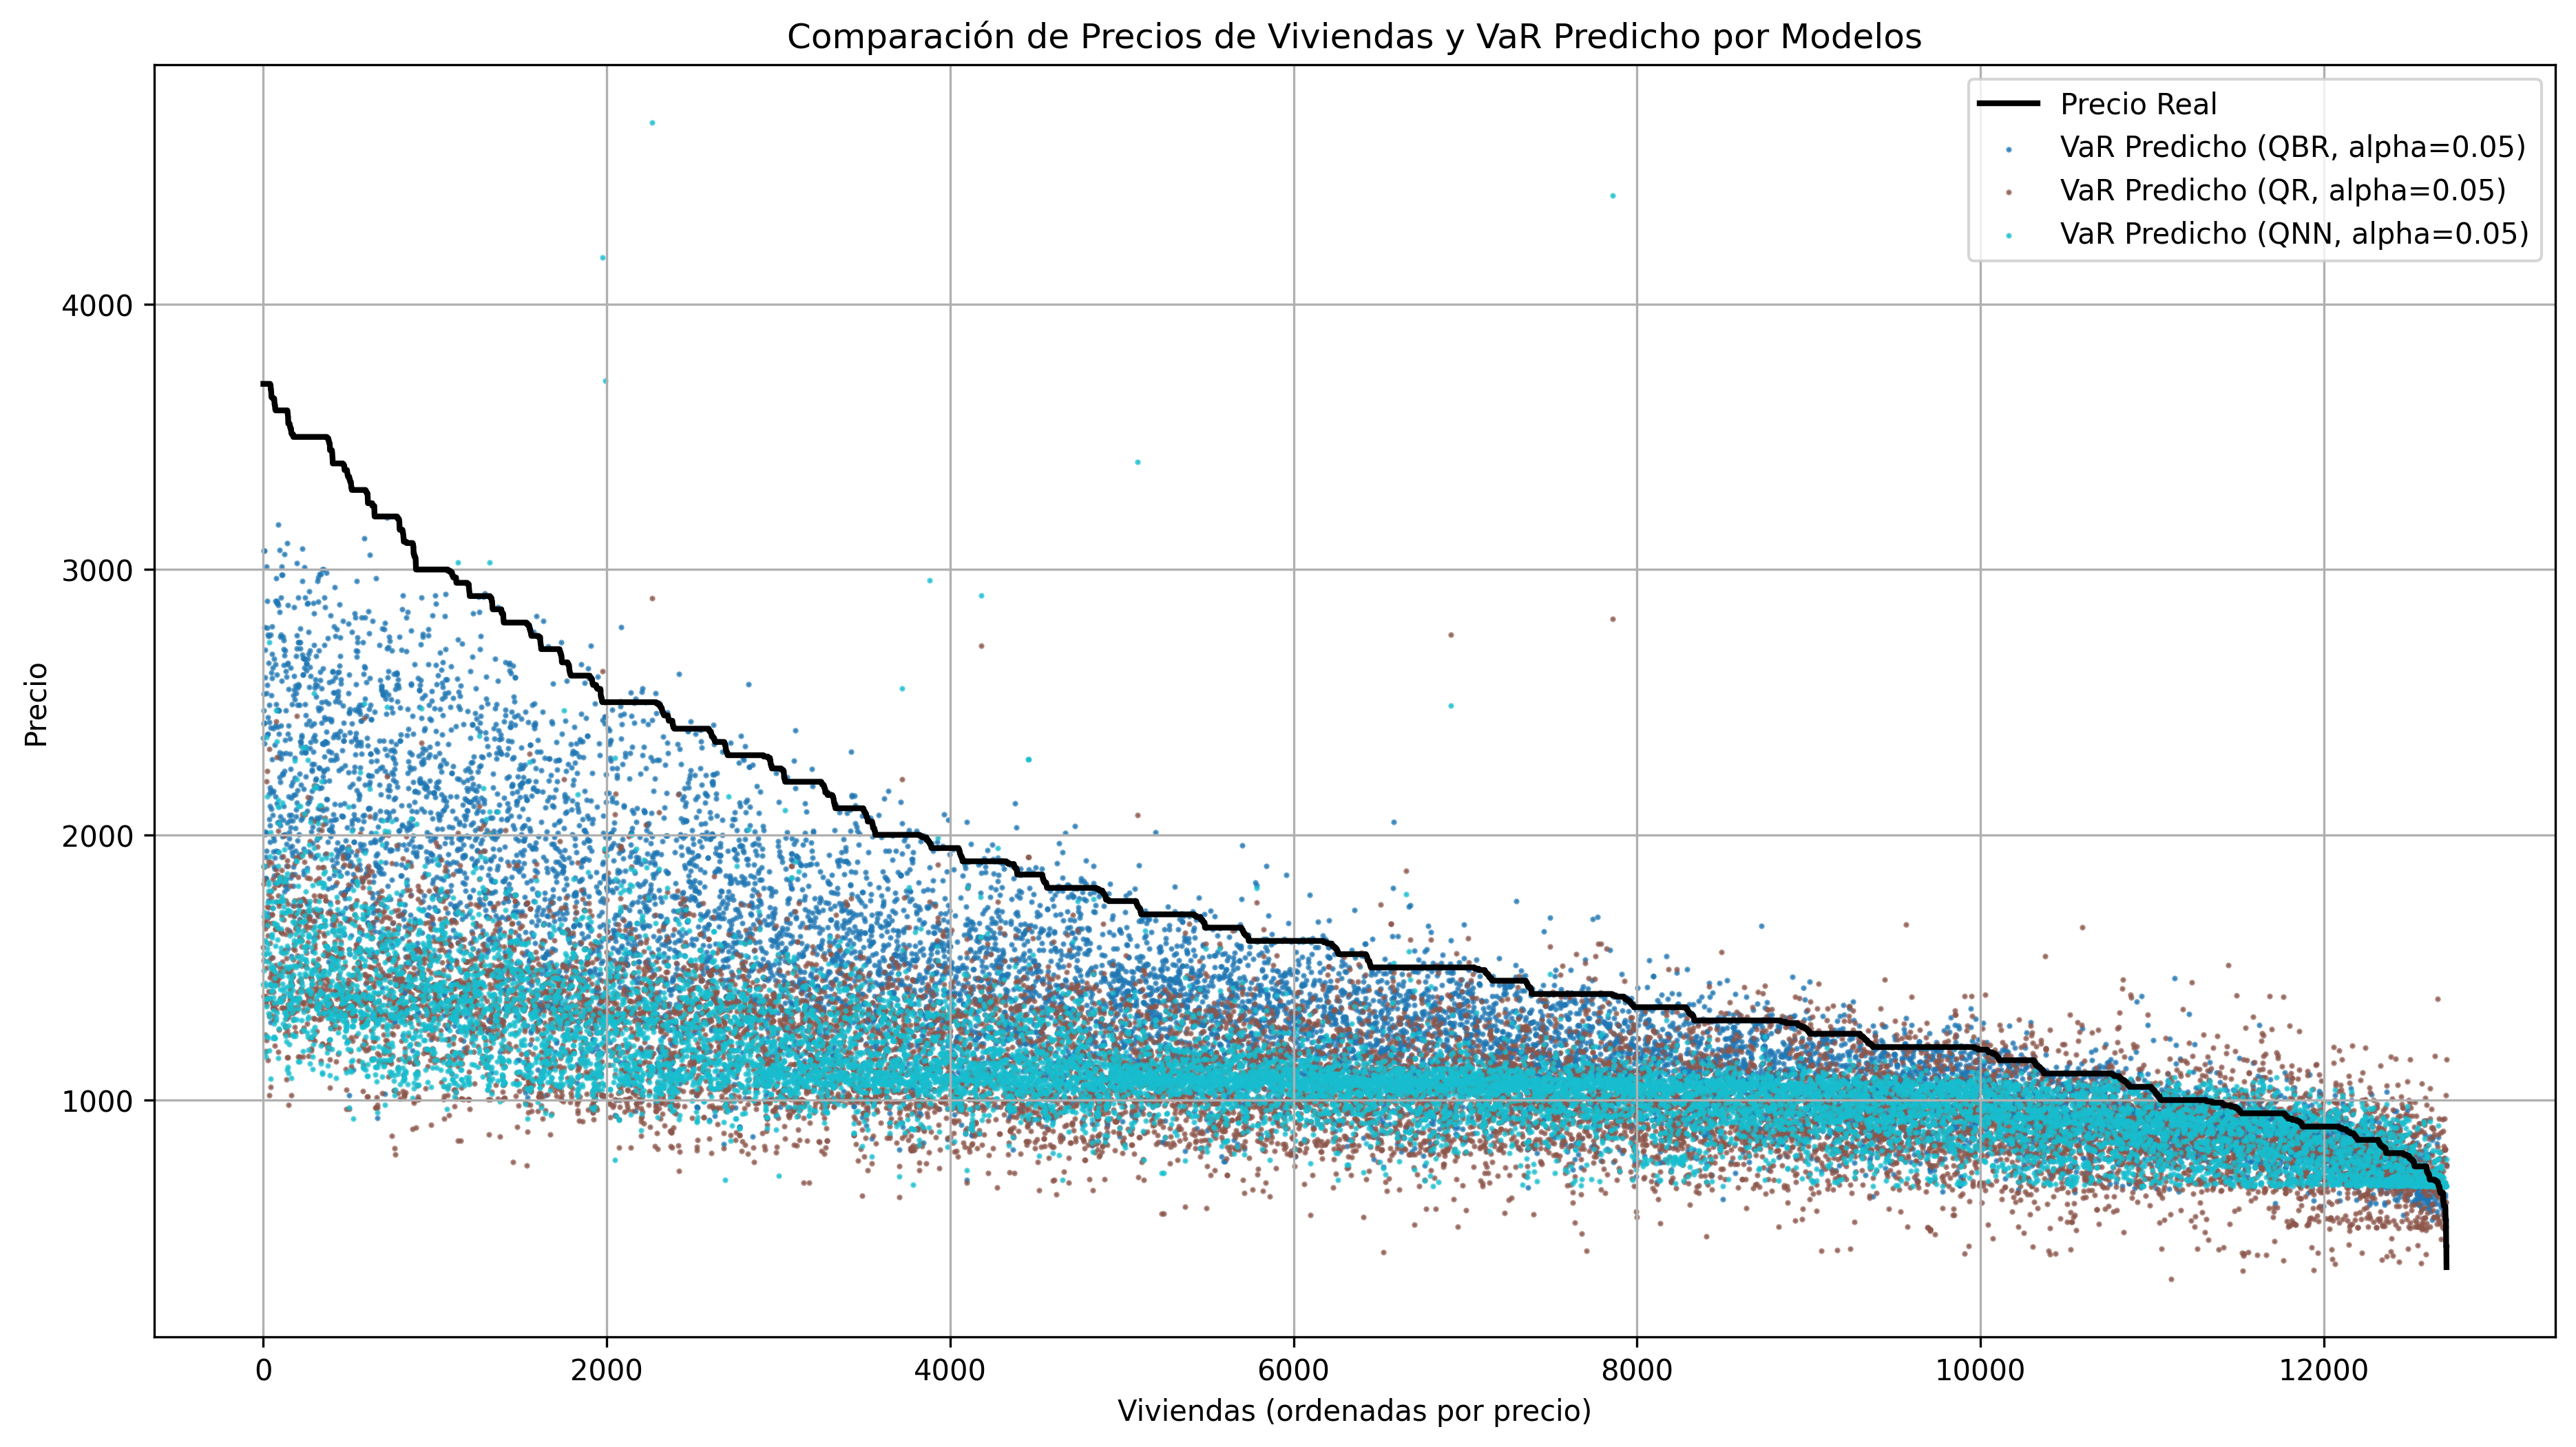
\includegraphics[width=0.95\textwidth]{prediction.png}
   \caption{Precios reales y el VaR estimado por los modelos QR, QNN y QBR para $\alpha=0.95$.}
   \label{fig:var_predictions}
\end{figure}










A pesar de que los tres modelos obtengan un resultado parecido, 
los resultados difieren. El modelo QBR, que 
ya se ha visto que era el más preciso, da la estimación más alta. Esto sugiere 
que ajusta de manera más óptima el riesgo específico de cada vivienda y 
es capaz de adaptarse a características particulares de la vivienda. En 
la figura~\ref{fig:var_error} se muestra el error de cada modelo al
predecir el VaR:
 \newpage

\begin{figure}[H]
   \centering
   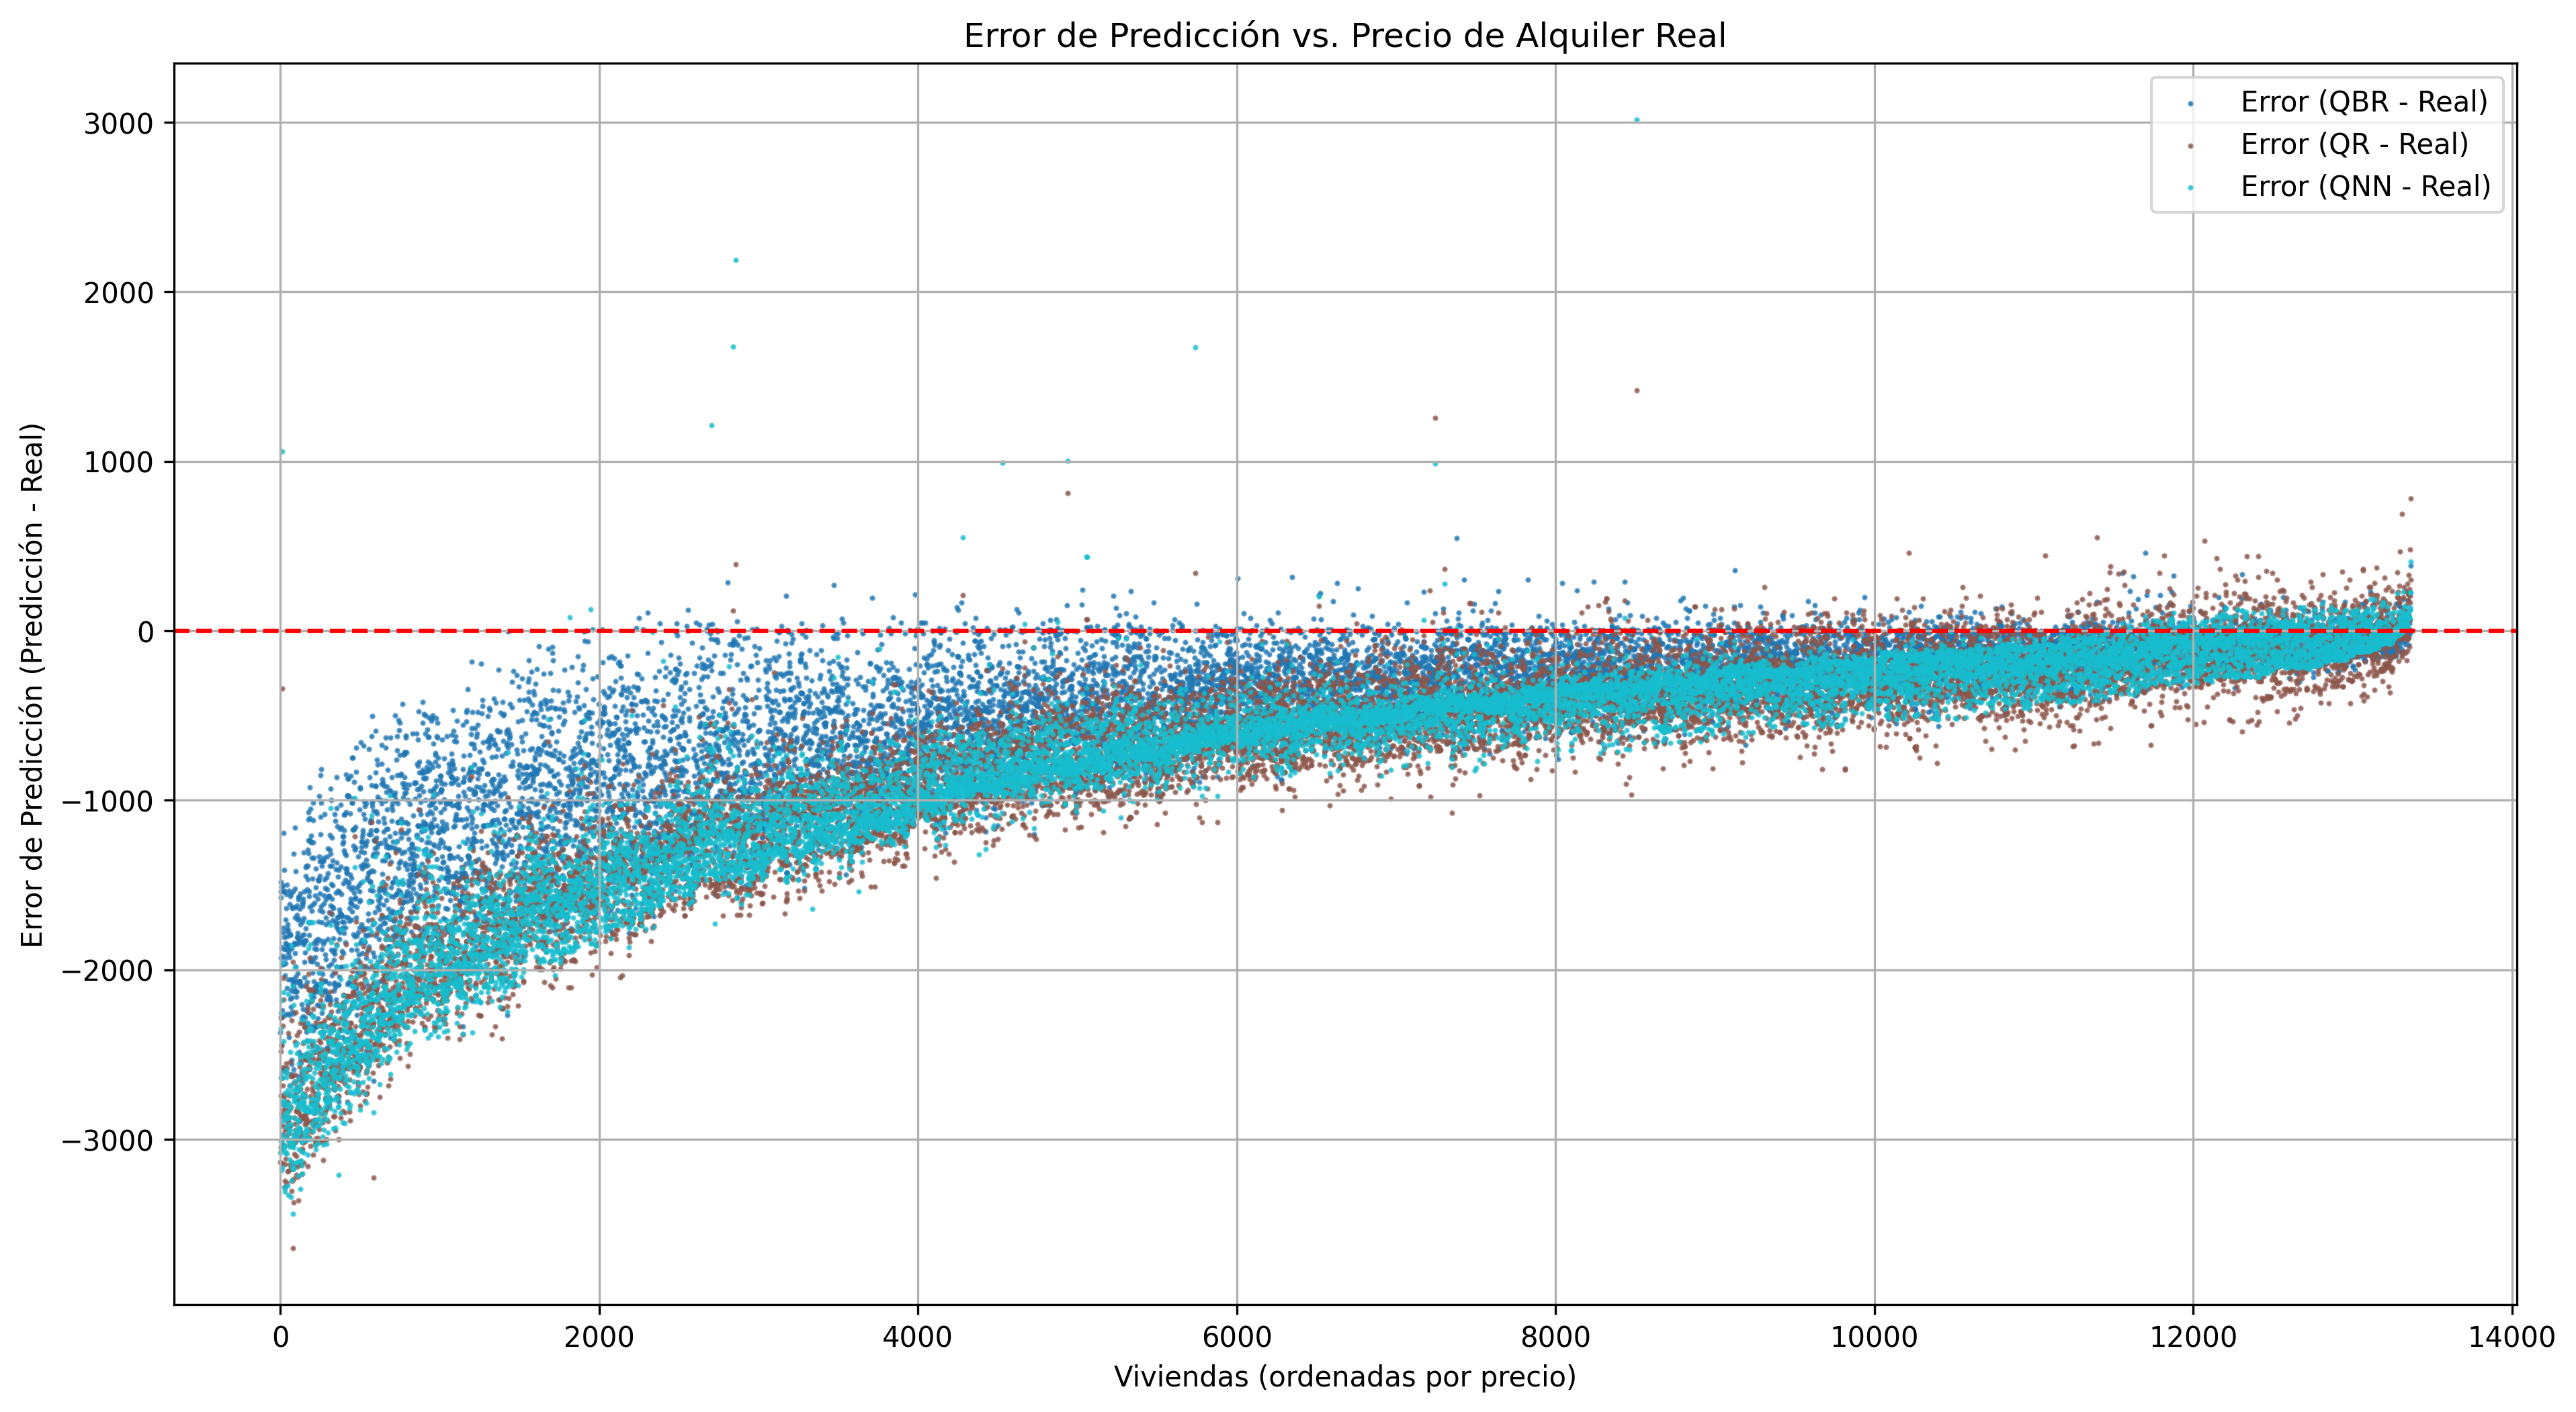
\includegraphics[width=0.95\textwidth]{errores_var.png}
   \caption{Error en la predicción VaR estimado por los modelos QR, QNN y QBR para $\alpha=0.95$.}
   \label{fig:var_error}
\end{figure}

Se puede observar que el boosting es más preciso en las colas de la distribución y que 
las tres predicciones se ajustan bastante bien  en la parte media y baja.\\


Una vez calculado el VaR, se va a calcular el Expected Shortfall (ES) para 
entender qué pasaría en el peor de los casos. En la figura~\ref{fig:es_predictions} se observa la 
distribución de los ES en función del par de métodos utilizados (combinación entre el método para calcular el cuantil y el expectil necesarios):
\newpage
\begin{figure}[H]
   \centering
   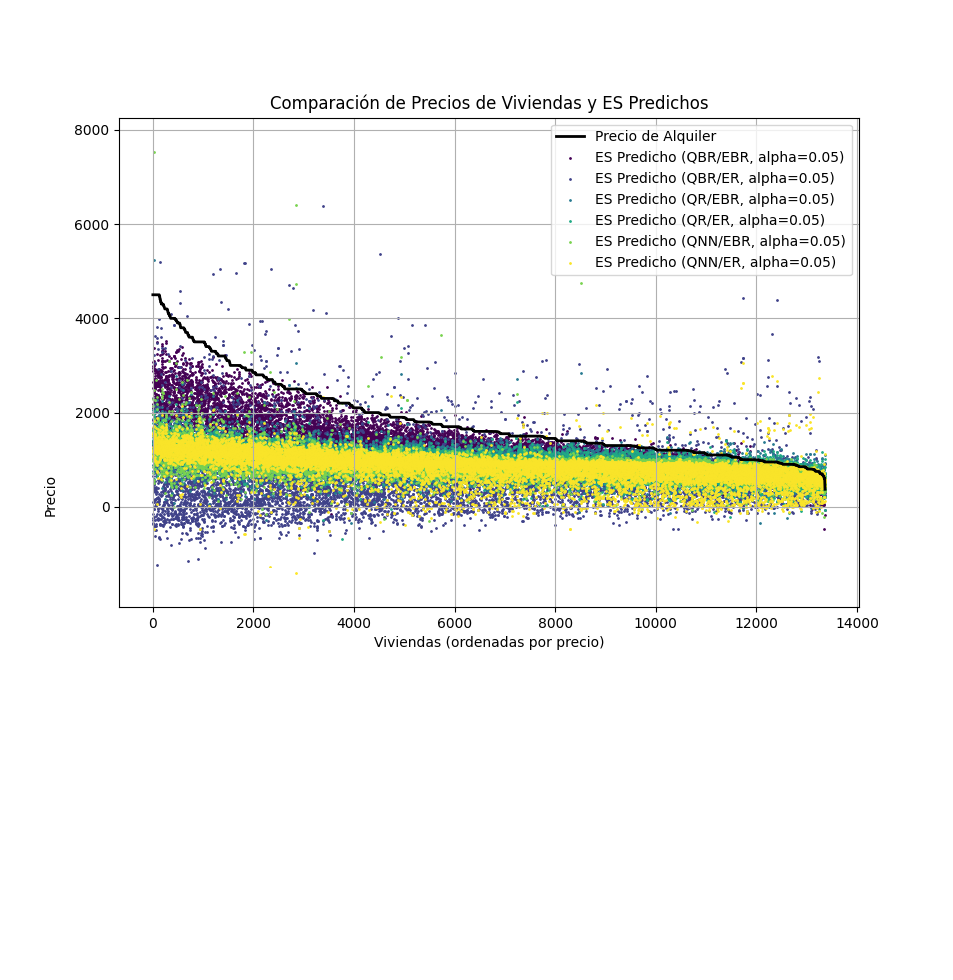
\includegraphics[width=0.95\textwidth]{es_predictions.png}
   \caption{Precios reales y el ES estimado por los modelos $\alpha=0.95$.}
   \label{fig:es_predictions}
\end{figure}

Se puede observar que los valores predichos están en su mayoría por debajo del precio del alquiler. Sin embargo, se puede ver alguna incorrección en algún cálculo, ya que esta inversión no puede tener retorno negativo y, sin embargo, se observa que el ES calculado en algunos casos es menor que 0. Esto se debe a que la precisión para calcular el cuantil es mayor que para calcular el expectil, lo cual hace que la estimación del ES se desvirtue.\\



\section{Caso de uso real}


Para ver cómo se comportan estos modelos en un caso práctico, se va a usar
cada uno para predecir la renta mínima de una vivienda concreta tomada de 
otro portal de viviendas~\cite{FC25}. Dicha vivienda se vende por 625000€ y 
se va a comprobar cuál es la renta mínima esperada al poner al alquiler dicha 
vivienda.
Los resultados se ven en la  Tabla~\ref{tab:var_predictions}.
 \newpage
 \begin{table}[h!]
   \centering
   \begin{tabular}{|l|c|}
      \hline
      \textbf{Modelo} & \textbf{Predicción de VaR (Renta Mínima Estimada)} \\
      \hline
      Regresión Cuantílica (QR) &  1235,09 €\\
      Red Neuronal Cuantílica (QNN) & 1135,35 € \\
      Boosting Cuantílico (QBR) &  1637,66€\\
      \hline
   \end{tabular}
   \caption{Predicción del VaR ($\alpha=0.95$) para la vivienda tomada como ejemplo.}
   \label{tab:var_predictions}
\end{table}
Por otro lado, también se obtienen la estimaciones del ES para este caso de uso:
 \begin{table}[h!]
   \centering
   \begin{tabular}{|l|c|}
      \hline
      \textbf{Modelo} & \textbf{Predicción de ES} \\
      \hline
        QR \& ER &  1071,38 €\\
      QR \& EBR  &  1134,49 €\\
      QBR \& ER &  233,81 €\\
      QBR \& EBR &  1619,22 €\\
      QNN \& ER &  951,29 €\\
      QNN \& EBR &  1014,39 €\\
      \hline
   \end{tabular}
   \caption{Predicción del ES ($\alpha=0.95$) para la vivienda tomada como ejemplo.}
   \label{tab:es_predictions}
\end{table}

Una vez obtenidos estos resultados, se puede hacer un 
cálculo de la rentabilidad mínima esperada de la inversión. Para ello, se ha 
consultado una web de cálculo de hipotecas~\cite{BBVA25} y se han obtenido 
los siguientes datos:
\begin{itemize}
   \item \textbf{Precio de la vivienda:} 625000€
   \item \textbf{Entrada:} 187500€ (30\% del precio de la vivienda)
   \item \textbf{Hipoteca:} 437500€ (70\% del precio de la vivienda)
   \item \textbf{Gastos aproximados de la compra:} 40228,31€
   \item \textbf{Intereses y gastos extra:} 2,74\%
   \item \textbf{Plazo:} 30 años
   \item \textbf{Cuota mensual:} 1728,45€
   \item \textbf{Intereses mensuales:} 513,37€
\end{itemize}
Para calcular la rentabilidad de una inversión inmobiliaria se debe tener en cuenta los ingresos netos que se van a percibir y los gastos totales asociados a la compra, sin considerar la parte de la hipoteca asociada a las amortizaciones del capital, ya que no representa un gasto real. Además del precio de compra/venta, se dispone de los valores de las variables explicativas utilizadas por los modelos predictivos, por lo que se usarán como entrada de los modelos ajustados para obtener una estimación del precio de alquiler. Por tanto, para calcular la rentabilidad anual, se aplica:
\begin{align*}
   r_{min} &= \frac{(\text{Ingresos mensuales}-\text{Gastos mensuales})*12}{\text{Entrada de la vivienda}+\text{Gastos asociados a la compra de la vivienda}} \\
\end{align*}

Por tanto, la rentabilidad mínima esperada de la inversión según el modelo 
que se escoja es la siguiente:
\begin{align*}
   r_{min}^{QBR} &= \frac{(1637.66 - 513,37)*12}{187500+40228,31} = 0,0592 = 5,92\% \\
   r_{min}^{QR} &= \frac{(1235.09 - 513,37)*12}{187500+40228,31} = 0,0380 = 3,80 \% \\
   r_{min}^{QNN} &= \frac{(1135.35 - 513,37)*12}{187500+40228,31} = 0,0327 = 3,27\% \\
\end{align*}

Por otro lado, también interesa saber la rentabilidad esperada en caso de 
que esta fuese menor a la mínima. En ese caso, se toma el ES:

\begin{align*}
    r_{min}^{QBR, EBR} &= \frac{(1619,22 - 513,37)*12}{187500+40228,31} = 0,0583 = 5,83\% \\
    r_{min}^{QR, EBR} &= \frac{(1134,49- 513,37)*12}{187500+40228,31} = 0,0258 = 2,58 \% \\
    r_{min}^{QNN, EBR} &= \frac{(1014,39 - 513,37)*12}{187500+40228,31} = 0,0327 = 3,27\% \\
    r_{min}^{QBR, ER} &= \frac{(233,81 - 513,37)*12}{187500+40228,31} = -0,0147 = -1.47\% \\
    r_{min}^{QR, ER} &= \frac{(1071,38 - 513,37)*12}{187500+40228,31} = 0,0294 = 2,94 \% \\
    r_{min}^{QNN, ER} &= \frac{(951,29 - 513,37)*12}{187500+40228,31} = 0,0231 = 2,31\% \\
\end{align*}

A pesar de no haberse tenido en cuenta gastos extra como la 
comunidad, el seguro de la vivienda y más, estos datos serían los que un
inversor podría utilizar para valorar si merece la pena o no la inversión. 
\clearemptydoublepage

%-------------
\backmatter                      % Parte final del texto



%------ Bibliografía
% Para meter cosas en el "toc" a mano, ver
% \S 2.3.1 del LaTeX Companion (ejemplo de la p. 47) (Juan Luis)
\phantomsection % Si no, el enlace en el índice apunta a la página anterior
\addcontentsline{toc}{chapter}{\bibname} % Para que salga en el índice general
% Para ponerlo a mano en la cabecera, pues no es \chapter:
\chaptermark{\bibname}
% Cuando no hay secciones para las cabeceras impares, se suele hacer esto:
\sectionmarkwithoutsections{\bibname}

%--- BIBLIOGRAFÍA DEL TFG
\begin{thebibliography}{99}

\bibitem{AT02a}
\textsc{C. Acerbi y D. Tasche},  
\textit{On the Coherence of Expected Shortfall},  
Journal of Banking \& Finance, 2002.

\bibitem{AT02b}
\textsc{C. Acerbi y D. Tasche},  
\textit{Expected Shortfall: A Natural Coherent Alternative to Value at Risk},  
Economic Notes, 2002.

\bibitem{BIS}
\textsc{Bank for International Settlements (BIS)},
\textit{Basel III: A global regulatory framework for more resilient banks and banking systems}, 
rev. June 2011,
\url{https://www.bis.org/publ/bcbs189.pdf}.


\bibitem{BBVA25}
\textsc{BBVA},
\textit{Simulador de hipotecas},
BBVA.es, consultado el 7 de julio de 2025, disponible en
\url{https://www.bbva.es/personas/productos/hipotecas/simulador-hipotecas.html}.

\bibitem{BFOS84}
\textsc{L. Breiman, J. H. Friedman, R. A. Olshen y C. J. Stone},  
\textit{Classification and Regression Trees},  
Wadsworth International Group, 1984.


\bibitem{FS08}
\textsc{H. Föllmer y A. Schied},
\textit{Convex and coherent risk measures}, 
Humboldt‑Universität zu Berlin, Institut für Mathematik;  
versión del 8 de octubre de 2008, disponible en  
\url{https://www.math.hu-berlin.de/~foellmer/papers/CCRM.pdf}.



\bibitem{FC25}
\textsc{Fotocasa},  
\textit{Anuncio de vivienda en venta en Madrid capital (ID: 185543795)},  
Fotocasa.es, consultado el 6 de julio de 2025, disponible en  
\url{https://www.fotocasa.es/es/comprar/vivienda/madrid-capital/aire-acondicionado-calefaccion-ascensor-no-amueblado/185543795/}.



\bibitem{Frazier18}
\textsc{P. I. Frazier},  
\textit{A Tutorial on Bayesian Optimization},  
2018, consultado el 8 de julio de 2025, disponible en  
\url{https://arxiv.org/pdf/1807.02811}.



\bibitem{HTF17}
\textsc{T. Hastie, R. Tibshirani y J. Friedman},  
\textit{The Elements of Statistical Learning: Data Mining, Inference, and Prediction}, Springer, 2017,  
disponible en \url{https://hastie.su.domains/ElemStatLearn/printings/ESLII_print12_toc.pdf.download.html}.


\bibitem{ID25}
\textsc{Idealista},
\textit{Datos de viviendas en alquiler en la provincia de Madrid},
Idealista.com, consultado el 5 de julio de 2025, disponible en  
\url{https://www.idealista.com/alquiler-viviendas/madrid-provincia/}.

\bibitem{IS15}
\textsc{S. Ioffe y C. Szegedy},  
\textit{Batch Normalization: Accelerating Deep Network Training by Reducing Internal Covariate Shift},  
Proceedings of the 32nd International Conference on Machine Learning (ICML), 2015, 
disponible en \url{http://static.googleusercontent.com/media/research.google.com/en//pubs/archive/43442.pdf}.

\bibitem{KB14}
\textsc{D. P. Kingma y J. Ba},  
\textit{Adam: A Method for Stochastic Optimization}, 2014
disponible en \url{https://arxiv.org/pdf/1412.6980}.

\bibitem{K05}
\textsc{R. Koenker},
\textit{Quantile Regression}, 
Cambridge University Press, 2005.



\bibitem{MC20}
\textsc{P. Martínez-Camblor},
\textit{Regresión Cuantilica: Estimación y Contrastes}, 
Universidad Autónoma de Madrid, 2020, disponible en  
\url{https://www.uam.es/uam/media/doc/1606862082401/regresion-cuantilica-estimacion-y-contrastes.pdf}.


\bibitem{NG04}
\textsc{A. Y. Ng},  
\textit{Feature selection, L1 vs. L2 regularization, and rotational invariance},  
Proceedings of the Twenty-First International Conference on Machine Learning (ICML), 2004,  
disponible en \url{https://robotics.stanford.edu/~ang/papers/icml04-l1l2.pdf}.

\bibitem{RM96}
\textsc{J.P. Morgan},
\textit{RiskMetrics — Technical Document},
4ª edición, J.P. Morgan/Reuters, Nueva York, 1996,  
consultado el 9 de julio de 2025, disponible en  
\url{https://www.msci.com/documents/10199/5915b101-4206-4ba0-aee2-3449d5c7e95a}.


\bibitem{NP87}
\textsc{W. K. Newey y J. L. Powell},
\textit{Asymmetric least squares estimation and testing}, 
Econometrica, 1987,
\url{https://doi.org/10.2307/1911031}.

\bibitem{KO17}
\textsc{K. K. Osmundsen},
\textit{Using Expected Shortfall for Credit Risk Regulation}, 
University of Stavanger, Stavanger, 26 de febrero de 2017.

\bibitem{OBU17}
\textsc{M. Osorio Buitrón},
\textit{Estimación del Valor en Riesgo (VaR) para la tasa de cambio (TRM) COP‑USD mediante modelos ARCH},  
Trabajo de grado en Estadística, Universidad del Valle, Santiago de Cali, Colombia, 2017,  
disponible en \url{https://bibliotecadigital.univalle.edu.co/server/api/core/bitstreams/9ce73714-c4c7-45ec-82ac-c46591f78c2f/content}.



\bibitem{SSU}
\textsc{S. Sarykalin, G. Serraino y S. Uryasev},
\textit{Value-at-Risk vs. Conditional Value-at-Risk in Risk Management and Optimization}, 
Tutorials in Operations Research, INFORMS, 2008,
\url{https://pubsonline.informs.org/doi/epdf/10.1287/educ.1080.0052}.



\bibitem{SF12}
\textsc{R. E. Schapire y Y. Freund},
\textit{Boosting: Foundations and Algorithms}, 
MIT Press, 2012,
\url{https://direct.mit.edu/books/book/5342/Boosting-Foundations-and-Algorithms}.

\bibitem{SHKSS14}
\textsc{N. Srivastava, G. Hinton, A. Krizhevsky, I. Sutskever y R. Salakhutdinov},  
\textit{Dropout: A Simple Way to Prevent Neural Networks from Overfitting},  
Journal of Machine Learning Research, vol. 15, pp. 1929–1958, 2014,  
disponible en \url{https://www.cs.toronto.edu/~rsalakhu/papers/srivastava14a.pdf}.



\bibitem{Taylor08}
\textsc{J.W. Taylor},  
\textit{Estimating Value at Risk and Expected Shortfall Using Expectiles},  
Journal of Financial Econometrics, vol. 6, n.º 2, 2008, pp. 231–252,  
disponible en  
\url{https://users.ox.ac.uk/~mast0315/ExpectilesVaR&ES.pdf}.










\end{thebibliography}
%--- FIN DE LA BIBLIOGRAFÍA

\clearemptydoublepage

\appendix
\renewcommand{\thechapter}{A\arabic{chapter}} % Para que salga A1, A2, etc.
\counterwithin{section}{chapter}
\renewcommand{\thesection}{\thechapter.\arabic{section}} % A1.1, A1.2...
\renewcommand{\thesubsection}{\thesection.\arabic{subsection}} % A1.1.1, etc.

\setcounter{chapter}{1}

\chapter{Apéndice 1: Árboles de regresión }
\label{ap:arboles}
Los árboles de regresión~\cite{BFOS84} son modelos predictivos no paramétricos 
que dividen el espacio de las variables de entrada en subregiones rectangulares disjuntas. 
Dentro de cada una de estas regiones, se ajusta un modelo simple para realizar 
predicciones. Este proceso de división se realiza de forma recursiva, creando 
una estructura jerárquica similar a un árbol.\\

El objetivo principal de un árbol de regresión es minimizar el error de 
predicción. Para ello, en cada paso de la construcción del árbol, se busca la 
mejor división posible de los datos. Una división se define por una variable 
predictora y un punto de corte y la "mejor" división es aquella que reduce al 
máximo una función de pérdida predefinida.\\ 

Se considera un conjunto de datos de entrenamiento con variables 
explicativas $\mathbf{X} = \{X_1, X_2, \dots, X_p\}$ y una variable dependiente 
$Y$. El proceso de construcción del árbol implica encontrar divisiones 
binarias recursivas. Para cada nodo del árbol, se evalúan todas las posibles 
variables $X_j$ y todos los posibles puntos de corte $t$ para esa variable, 
con el fin de encontrar la división que optimice la función de pérdida. 
Por ejemplo, para la función de pérdida cuadrática, la división se 
realizaría de la siguiente manera
\begin{align*}
   \mathcal{L}(X_j, t) = \sum_{i=1}^n I(X_{ij} \leq t) (Y_i - \bar{Y}_{X_{ij} \leq t})^2 + \sum_{i=1}^n I(X_{ij} > t)(Y_i - \bar{Y}_{X_{ij} > t})^2
\end{align*}
donde $\bar{Y}_{X_i \leq t}$ y $\bar{Y}_{X_i > t}$ son las medias de $Y$ en las 
regiones definidas por la división. Esta recursividad se repite hasta que se 
cumplen ciertos criterios de parada, como una profundidad máxima del árbol 
o un  número mínimo de observaciones en un nodo. \\

Para los casos explorados en este trabajo, se han utilizado árboles de 
regresión binarios como predictores débiles del algoritmo de boosting. 
Estos árboles se han construido utilizando el proceso presentado, adaptando 
la función de pérdida. En el caso del boosting para cuantiles, se 
ha intentado minimizar la suma de las pérdidas pinball en cada región, es decir:
\begin{align*}
   \mathcal{L}(X_j, t) = \sum_{i \in R_1(j,t)} \rho_\alpha(Y_i - c_1) + \sum_{i \in R_2(j,t)} \rho_\alpha(Y_i - c_2)
\end{align*}
donde $R_1(j,t)$ y $R_2(j,t)$ son las dos regiones resultantes de la división por la variable 
$X_j$ en el punto de corte $t$, y $c_1$ y $c_2$ son las predicciones óptimas (cuantiles 
condicionales) para cada región.

Mientras que para el caso de los expectiles, se ha intentado minimizar la suma de las 
pérdidas expectílicas en cada región:
\begin{align*}
   \mathcal{L}(X_j, t) = \sum_{i \in R_1(j,t)} \phi_\tau(Y_i - e_1) + \sum_{i \in R_2(j,t)} \phi_\tau(Y_i - e_2)
\end{align*}
donde $e_1$ y $e_2$ son las predicciones óptimas (expectiles condicionales) para 
cada región.\\

Una vez el árbol está construido, se puede realizar una predicción dados la introducción de 
un nuevo dato. El dato se introduce en el árbol desde el nodo raíz y, siguiendo las 
subdivisiones, llegará a una hoja. La predicción se realiza de forma distinta 
dependiendo si se quiere el cuantil o el expectil. Se supone el conjunto de 
variables que caen en la hoja $\{Y_i\}_{i \in R}$, donde $R$ es el conjunto de
índices de las observaciones que caen en la hoja. Para calcular el cuantil de la hoja 
se toma el cuantil de las observaciones que caen en la hoja:
\begin{align*}
   \hat{q}_\alpha = Y_{(\lceil \alpha \cdot n_h \rceil)}
\end{align*}
Por otro lado, el expectil se calcula mediante el 
algoritmo Iteratively Reweighted Least Squares (IRLS) presentado 
por Newey y Powell~\cite{NP87}.

\section{Ventajas y desventajas de los árboles de regresión}
Los árboles de regresión son una herramienta muy poderosa y tiene unas 
grandes ventajas, pero también se pueden encontrar deficiencias:

\subsubsection*{Ventajas}
\begin{itemize}
    \item \textbf{Facilidad de Interpretación:} Son modelos muy  fáciles de 
    entender, ya que su estructura se parece a un diagrama de flujo de 
    decisiones.
    \item \textbf{Manejo de Relaciones No Lineales:} Pueden capturar 
    relaciones complejas y no lineales entre las variables sin necesidad de 
    transformaciones previas de los datos.
    \item \textbf{No Requieren Normalización:} No es necesario escalar o 
    normalizar las variables de entrada, simplificando la preparación de los datos.
    \item \textbf{Robustez ante Valores Atípicos:} Son robustos ante la presencia 
    de valores atípicos en los datos.
    \item \textbf{Selección Automática de Características:} Realizan una 
    selección automática de las características más relevantes al elegir las 
    mejores divisiones.
\end{itemize}

\subsubsection*{Desventajas}
\begin{itemize}
   \item \textbf{Sobreajuste:} Son propensos al sobreajuste, sobre todo si los 
   datos son ruidosos o el árbol muy profundo. Más adelante se exploran 
   técnicas para evitarlo.
   \item \textbf{Inestabilidad:} Pequeñas variaciones en el conjunto de 
   datos pueden dar lugar a árboles muy diferentes, lo que 
   puede afectar a la generalización del modelo.
   \item \textbf{Sesgo hacia Divisiones con Muchas Características:} Pueden
   favorecer divisiones que involucran muchas características, lo que puede
   llevar a una interpretación errónea de la importancia de las variables.
\end{itemize}



\setcounter{chapter}{2}
\setcounter{section}{0}


\chapter{Apéndice 2: Detalles de los algoritmos de optimización de los modelos}
\label{ap:optimizacion}
Con el objetivo de mejorar la precisión de los modelos, se han utilizado 
diferentes algoritmos de optimización para ajustar los parámetros asociados 
a cada modelo. Cada uno de ellos ha aportado una gran mejoría al rendimiento 
del modelo. Esto ha sido especialmente relevante en el caso de las 
redes neuronales, donde la optimización de los pesos y sesgos es crucial.
\section{Reescalado y normalización de los datos}
Para mejorar la convergencia de los algoritmos de optimización, se ha
optado por aplicar un reescalado y normalización de los datos, lo cual 
facilita el entrenamiento de todos los modelos. Para cada variable se realiza 
la siguiente transformación: 
\begin{align*}
   x_{scaled} = \frac{x - \mu}{\sigma}
\end{align*}
donde $\mu$ es la media de la variable y $\sigma$ es su desviación estándar. 
%\clearemptydoublepage
\section{Técnicas de regularización}
Las regularizaciones son técnicas utilizadas para evitar el sobreajuste 
y hacer que el modelo
se centre más en la tendencia general, en lugar 
de ajustar el ruido de los datos. Es muy frecuente observar en los modelos 
sobreajustados coeficientes o pesos con magnitudes elevadas, por esto 
una forma de mitigar el sobreajuste consiste en penalizar los modelos con 
coeficientes muy grandes. 
Se han utilizado técnicas de regularización L1 y L2~\cite{NG04}, que penalizan
los pesos del modelo para evitar que se vuelvan demasiado grandes.
Para lograrlo, se intenta minimizar una función de pérdida que incluye un 
término de regularización. Las funciones de pérdida incluyendo las 
regularizaciones L1 y L2 son las siguientes:
\begin{align*}
   \mathcal{L}_{L1}(\mathbf{X_i}, \mathbf{Y}_i, g) &= \sum_{i=1}^m \rho(\mathbf{Y}_i - f(\mathbf{X}_i)) + \upsilon \sum_{j=1}^n |w_j| \\
   \mathcal{L}_{L2}(\mathbf{X_i}, \mathbf{Y}_i, g) &= \sum_{i=1}^m \rho(\mathbf{Y}_i - f(\mathbf{X}_i)) + \lambda \sum_{j=1}^n w_j^2 \\
   \mathcal{L}_{L1+L2}(\mathbf{X_i}, \mathbf{Y}_i, g) &= \sum_{i=1}^m \rho(\mathbf{Y}_i - f(\mathbf{X}_i)) + \upsilon \sum_{j=1}^n |w_j| + \lambda \sum_{j=1}^n w_j^2
\end{align*}
con $\upsilon$ y $\lambda$ los parámetros de regularización L1 y L2, 
respectivamente, y $w_j$ todos los pesos del modelo. Al ser el objetivo 
minimizar la función de pérdida, el modelo trata de encontrar un equilibrio 
entre ajustar los datos y mantener los pesos con pequeños valores, 
lo cual ayuda a mejorar la sensibilidad a datos atípicos y la generalización 
del modelo.\\

Por otro lado, en las redes neuronales se utiliza una técnica llamada 
Dropout~\cite{SHKSS14} . Por cada entrada de datos en el entrenamiento, 
se desactivarán de forma aleatoria un porcentaje de las neuronas de la red. 
Con esto se consigue que la red, por una parte, reducir el sobreajuste y 
que determinadas neuronas no se vuelvan demasiado importantes y, 
por otra parte, simula un entrenamiento de múltiples modelos que, 
combinados, forma un modelo más robusto.\\

También, en las redes neuronales, se utiliza la normalización por 
lotes (Batch Normalization)~\cite{IS15}, que consiste en normalizar las 
activaciones de cada capa de la red. Esto ayuda a estabilizar el entrenamiento 
y acelerarlo, ya que reduce la variación en la distribución
de las entradas a cada capa a medida que cambian los pesos de las 
capas anteriores. 

\section{Búsqueda de hiperparámetros: la Búsqueda Bayesiana}
La correcta elección de los hiperparámetros es una de las claves para 
el éxito de un modelo de machine learning. Existen muchas técnicas para 
escogerlos. La que ofrece mejor rendimiento es la búsqueda de cuadrícula 
(Grid Search), que consiste en probar todas las combinaciones posibles de los
hiperparámetros y escoger la que mejor rendimiento tenga. Sin embargo,
es muy costosa computacional y temporalmente, por lo que 
se debe utilizar alguna otra técnica que pueda optimizarlos más 
eficientemente. \\ 

En este caso, se ha utilizado la búsqueda bayesiana~\cite{Frazier18}. Este 
método consiste en optimizar una función objetivo mediante la 
construcción de un modelo probabilístico que representa la función. Se ha 
optado por este método debido a que tiene una gran corrección cuando 
los hiperparámetros no superan un número razonable (en este caso,
menos de 10). \\ 

Para ejemplificar el algoritmo de búsqueda bayesiana, se define un espacio 
de hiperparámetros $\mathcal{X}$, y un conjunto de combinaciones iniciales 
de hiperparámetros $\{\kappa_1, \kappa_2, \dots, \kappa_{n_0}\} \subset \mathcal{X}$, 
generadas aleatoriamente.\\

Sea $f(\kappa)$ la función objetivo que se quiere optimizar, que evalúa la 
configuración de hiperparámetros $\kappa \in \mathcal{X}$.  Además, se define 
una función de adquisición $a(\kappa \mid \mathcal{D})$ de la siguiente manera:
\begin{align*}
   a(\kappa \mid \mathcal{D}) = \mathbb{E} \left[ \max(f_{\text{mejor}} - f(\kappa), 0) \right]
\end{align*}
con $\mathcal{D}$ el conjunto de observaciones de la función objetivo y
$f_{\text{mejor}}$ el mejor valor de la función objetivo encontrado hasta el 
momento.\\

\begin{algorithm}[H]
\caption{Búsqueda Bayesiana}
Inicializar el conjunto de observaciones $\mathcal{D} = \{\}$\;
Definir una distribución a priori sobre la función objetivo $f(\kappa)$, 
que modela nuestra creencia inicial sobre su comportamiento 
(proceso gaussiano con media y covarianza predefinidas)\;
Generar $n_0$ configuraciones iniciales $\kappa_1, \dots, \kappa_{n_0} \in \mathcal{X}$ aleatoriamente\;

\For{$i = 1$ \KwTo $n_0$}{
    Evaluar $y_i = f(\kappa_i)$\;
    Añadir $(\kappa_i, y_i)$ a $\mathcal{D}$\;
}

\For{$i = n_0+1$ \KwTo $N$}{
    Actualizar la distribución de probabilidad a posteriori sobre $f$ utilizando 
    todos los datos disponibles $\mathcal{D}$\;
    Construir la función de adquisición $a(\kappa \mid \mathcal{D})$\;
    Seleccionar los siguientes hiperparámetros:
    \begin{align*}
      \kappa_i = \arg\max_{\kappa \in \mathcal{X}} a(\kappa \mid \mathcal{D})      
    \end{align*}
    
    Evaluar $y_i = f(\kappa_i)$\;
    Añadir $(\kappa_i, y_i)$ a $\mathcal{D}$\;
}
\end{algorithm}
\setcounter{chapter}{3}
\setcounter{section}{0}

\chapter{Apéndice 3: Código utilizado en Python y R}
\section{Implementación de modelos en Python}
\begin{lstlisting}[style=pythonstyle, caption=main.py]
   from ml.expectileboosting import EBR
from ml.quantileboosting import QBR
from ml.neuralnetwork import QuantileNeuralNetwork
from regression.quantileregression import QR 
from regression.expectileregression import ER 
import matplotlib.cm as cm
import numpy as np 
import matplotlib.pyplot as plt 
from sklearn.preprocessing import StandardScaler
import pandas as pd
import time


class ModelPredictor: 
    def __init__(self, X, y):
        self.qbr = QBR(X, y)
        self.qr = QR(X, y)
        self.qnn  = QuantileNeuralNetwork(X, y)
        self.er = ER(X, y)
        self.ebr = EBR(X, y)
    
    def fit_quantile_models(self, alpha:float):
        self.qbr.fit(alpha)
        self.qr.fit(alpha)
        self.qnn.fit(alpha)

    def fit_expectile_models(self):
        for t in range(1, 100):
            t = t/100
            self.ebr.fit(t)
            self.er.fit(t)
            
        

    ###Hallamos el VaR con todas las tecnicas###
    def predict_VaR(self, method: str, X_scalar, alpha:float): 
        if method == "QBR":
            return self.qbr.predict(alpha, X_scalar)
        elif method == "QR": 
            return self.qr.predict(alpha, X_scalar)
        elif method == "QNN":
            return self.qnn .predict(alpha, X_scalar)
        
    def predict_ES_scalar(self, method: str, X_scalar:float, alpha: float, predicted_VaR_scalar:float, y):
        if method == "EBR":
            model = self.ebr
        elif method == "ER": 
            model = self.er 

        ##Hay que hallar el tau que corresponde al VaR
        min_diff = float("inf")
        expectile = None
        tau = None

        # Buscamos el tau que minimiza la diferencia entre el VaR predicho y expectil
        for t in range (1, 100):
            t = t/100
            exp = model.predict(t, X_scalar.reshape(1, -1))
            if abs(exp - predicted_VaR_scalar) < min_diff:
                min_diff = abs(exp - predicted_VaR_scalar)
                expectile = exp 
                tau = t
            else: 
                break 
        if tau == 0.5:
            print("Warning: tau is  0.5, this might indicate an issue with the model or data.")
            return 0
        
        ES = predicted_VaR_scalar + tau/(alpha*(2*tau-1))*(model.predict(0.5, X_scalar.reshape(1, -1))-predicted_VaR_scalar)
        return ES


    def predict_ES(self, method: str, X, alpha: float, predicted_VaR:float, y):
        ES = np.zeros(len(X))
        for i in range(len(X)): 
            ES[i] = self.predict_ES_scalar(method, X_scalar = X[i], alpha = alpha, predicted_VaR_scalar = predicted_VaR[i], y = y)
        return ES
    
    def VaR_Score(self, method: str, X, y, alpha: float):
        if method == "QBR":
            return self.qbr.score(alpha, X, y)
        elif method == "QR":
            return self.qr.score(alpha, X, y)
        elif method == "QNN":
            return self.qnn.score(alpha, X, y)
        
    def ES_Score(self, method: str, X, y, alpha: float):
        if method == "EBR":
            model = self.ebr
        elif method == "ER":
            model = self.er
        return model.score(alpha, X, y)

 


if __name__ == "__main__":
    # Campos del archivo cleaned_rental_data.csv:
    # precio: Precio del alquiler (variable objetivo)
    # metros_cuadrados_construidos: Metros cuadrados construidos de la propiedad
    # habitaciones: Número de habitaciones
    # banos: Número de baños
    # planta: Planta en la que se encuentra la propiedad (0 para bajo, -1 para sótano, etc.)
    # latitud: Latitud de la ubicación de la propiedad
    # longitud: Longitud de la ubicación de la propiedad
    # ascensor: Si la propiedad tiene ascensor (1 si sí, 0 si no)
    # obra_nueva: Si la propiedad es de obra nueva (1 si sí, 0 si no)
    # piscina: Si la propiedad tiene piscina (1 si sí, 0 si no)
    # terraza: Si la propiedad tiene terraza (1 si sí, 0 si no)
    # parking: Si la propiedad tiene parking (1 si sí, 0 si no)
    # parking_incluido_en_el_precio: Si el parking está incluido en el precio (1 si sí, 0 si no)
    # aire_acondicionado: Si la propiedad tiene aire acondicionado (1 si sí, 0 si no)
    # trastero: Si la propiedad tiene trastero (1 si sí, 0 si no)
    # jardin: Si la propiedad tiene jardín (1 si sí, 0 si no)
    # planta_was_nan: Si el valor de la planta original era NaN (1 si sí, 0 si no)

    new_house = [73, 3, 1, 5, 40.418395, -3.677125, 1, 0, 0, 1, 0, 0, 1, 0, 0, 0]

    df = pd.read_csv("/home/hugonaudin/Documentos/UNI/24-25/TFG/codigo/credits/rental_data/cleaned_rental_data.csv", sep=',', encoding='utf-8-sig')
    y = df["precio"]
    X = df.drop(columns=["precio"]).values
#
    scaler = StandardScaler()
    X_scaled = scaler.fit_transform(X)
    modelpredictor = ModelPredictor(X_scaled,y)

    modelpredictor.fit_quantile_models(0.05)
    modelpredictor.fit_expectile_models()
#
    quantile_types = ["QBR", "QR", "QNN"]
    expectile_types = ["EBR", "ER"]
    VaR_score = {}
    ES_score = {}
    predictions_for_plot = {}
    predictions_ES_for_plot = {}
#
    for quantile_type in quantile_types:
        predicted_VaR = modelpredictor.predict_VaR(quantile_type, X_scaled, 0.05)
        predictions_for_plot[quantile_type] = predicted_VaR
        VaR_score[quantile_type] = modelpredictor.VaR_Score(quantile_type, X_scaled, y, 0.05)

    print("VaR Scores:")
    for quantile_type, score in VaR_score.items():
        print(f"{quantile_type}: {score}")
   

    df = pd.read_csv("rental_data/cleaned_rental_data.csv", sep=',', encoding='utf-8-sig')
    
    y = df["precio"]
    X = df.drop(columns=["precio"]).values
    scaler = StandardScaler()
    X_scaled = scaler.fit_transform(X)
    modelpredictor = ModelPredictor(X_scaled,y)

    modelpredictor.fit_quantile_models(0.05)
    modelpredictor.fit_expectile_models()

    for quantile_type in quantile_types:
        predicted_VaR = modelpredictor.predict_VaR(quantile_type, X_scaled, 0.05)
        predictions_for_plot[quantile_type] = predicted_VaR
        VaR_score[quantile_type] = modelpredictor.VaR_Score(quantile_type, X_scaled, y, 0.05)


    print("VaR Scores:")
    for quantile_type, score in VaR_score.items():
        print(f"{quantile_type}: {score}")

    # --- Creación de la gráfica ---
    plot_df = pd.DataFrame({'Rent Price': y})
    for model, predictions in predictions_for_plot.items():
        plot_df[f'{model} VaR'] = predictions

    # Ordenar para graficar
    plot_df_sorted = plot_df.sort_values(by='Rent Price', ascending=False).reset_index(drop=True)

    # Configurar figura
    plt.figure(figsize=(15, 8))

    # Línea de precios reales
    plt.plot(
        plot_df_sorted.index,
        plot_df_sorted['Rent Price'],
        label='Precio de Alquiler',
        color='black',
        linewidth=2
    )

    # Colormap para asignar colores distintos automáticamente
    cmap = cm.get_cmap('tab10', len(predictions_for_plot))

    # Pintar cada modelo con color distinto
    for idx, model in enumerate(predictions_for_plot.keys()):
        plt.scatter(
            plot_df_sorted.index,
            plot_df_sorted[f'{model} VaR'],
            label=f'VaR Predicho ({model}, alpha=0.05)',
            color=cmap(idx),
            s=1, #puntos más pequeños 
            alpha=0.7
        )

    plt.title('Comparación de Precios de Viviendas y VaR Predicho por Modelos')
    plt.xlabel('Viviendas (ordenadas por precio)')
    plt.ylabel('Precio')
    plt.legend()
    plt.grid(True)

    plt.savefig("grafico_var_vs_precio2.png", dpi=300, bbox_inches='tight')
    plt.show()
    # --- Fin de la gráfica ---


    # --- Creación de la gráfica de errores ---
    plot_df = pd.DataFrame({'Rent Price': y})
    for model, predictions in predictions_for_plot.items():
        plot_df[f'{model} VaR'] = predictions

    # Ordenar para graficar
    plot_df_sorted = plot_df.sort_values(by='Rent Price', ascending=False).reset_index(drop=True)

    # Configurar figura
    plt.figure(figsize=(15, 8))

    # Colormap para asignar colores distintos automáticamente
    cmap = cm.get_cmap('tab10', len(predictions_for_plot))

    # Pintar cada modelo con color distinto
    for idx, model in enumerate(predictions_for_plot.keys()):
        error = plot_df_sorted[f'{model} VaR'] - plot_df_sorted['Rent Price']
        plt.scatter(
            plot_df_sorted.index,
            error,
            label=f'Error ({model} - Real)',
            color=cmap(idx),
            s=1,
            alpha=0.7
        )

    plt.title('Error de Predicción vs. Precio de Alquiler Real')
    plt.xlabel('Viviendas (ordenadas por precio)')
    plt.ylabel('Error de Predicción (Predicción - Real)')
    plt.legend()
    plt.grid(True)
    plt.axhline(y=0, color='r', linestyle='--') # Add a horizontal line at y=0 to see the error bias

    plt.savefig("grafico_errores_prediccion.png", dpi=300, bbox_inches='tight')
    plt.show()
    # --- Fin de la gráfica ---


    ##predecir el precio de new_house
    new_house = np.array(new_house).reshape(1, -1)
    scaled_new_house = scaler.transform(new_house)

    print("Predicted VaR for new house at 0.05:", modelpredictor.predict_VaR("QBR", scaled_new_house, 0.05))
    print("Predicted VaR for new house at 0.05:", modelpredictor.predict_VaR("QR", scaled_new_house, 0.05))
    print("Predicted VaR for new house at 0.05:", modelpredictor.predict_VaR("QNN", scaled_new_house, 0.05))

    print("\n\n--- ES Calculation ---")
    for quantile_type in quantile_types:
        predicted_VaR = modelpredictor.predict_VaR(quantile_type, scaled_new_house, 0.05)
        print(f"\nCalculating ES for VaR from {quantile_type} (VaR = {predicted_VaR}")
        for expectile_type in expectile_types:
            predicted_ES = modelpredictor.predict_ES_scalar(
                method=expectile_type,
                X_scalar=scaled_new_house[0],
                alpha=0.05,
                predicted_VaR_scalar=predicted_VaR[0],
                y=y
            )
            score = modelpredictor.ES_Score(expectile_type, X_scaled, y, 0.05)
            print(f"  - With {expectile_type} and {quantile_type}:  (ES: {prediected_ES:.2f})")


    # --- Calculation of ES for all data points ---
    es_predictions_for_plot = {}
    for quantile_type in quantile_types:
        predicted_VaR = predictions_for_plot[quantile_type]
        for expectile_type in expectile_types:
            print(f"Calculating ES for {quantile_type} and {expectile_type}")
            predicted_ES = modelpredictor.predict_ES(
                method=expectile_type,
                X=X_scaled,
                alpha=0.05,
                predicted_VaR=predicted_VaR,
                y=y
            )
            es_predictions_for_plot[(quantile_type, expectile_type)] = predicted_ES

    # --- Create plot with ES ---
    plot_df = pd.DataFrame({'Rent Price': y})
    for model, predictions in predictions_for_plot.items():
        plot_df[f'{model} VaR'] = predictions

    for (q_model, e_model), predictions in es_predictions_for_plot.items():
        plot_df[f'ES ({q_model}/{e_model})'] = predictions

    # Sort to plot
    plot_df_sorted = plot_df.sort_values(by='Rent Price', ascending=False).reset_index(drop=True)

    # Configure figure
    plt.figure(figsize=(15, 8))

    # Real prices line
    plt.plot(
        plot_df_sorted.index,
        plot_df_sorted['Rent Price'],
        label='Precio de Alquiler',
        color='black',
        linewidth=2
    )


    # Colormap for ES
    cmap_es = cm.get_cmap('viridis', len(es_predictions_for_plot))

    # Plot each ES model
    for idx, ((q_model, e_model), _) in enumerate(es_predictions_for_plot.items()):
        plt.scatter(
            plot_df_sorted.index,
            plot_df_sorted[f'ES ({q_model}/{e_model})'],
            label=f'ES Predicho ({q_model}/{e_model}, alpha=0.05)',
            color=cmap_es(idx),
            s=1, # Make ES points larger to distinguish them
        )

    plt.title('Comparación de Precios de Viviendas y ES Predichos')
    plt.xlabel('Viviendas (ordenadas por precio)')
    plt.ylabel('Precio')
    plt.legend()
    plt.grid(True)

    plt.savefig("grafico_es_vs_precio.png", dpi=300, bbox_inches='tight')
    plt.show()
    # --- End of ES plot ---

 \end{lstlisting}

 
\begin{lstlisting}[style=pythonstyle, caption=quantileregression.py]
   from sklearn.model_selection import KFold
from sklearn.linear_model import QuantileRegressor
from sklearn.model_selection import GridSearchCV
from sklearn.model_selection import train_test_split
from sklearn.metrics import make_scorer, mean_pinball_loss




class QR:
    def __init__(self, X, y ):
        self.X_train, self.X_test,self. y_train, self.y_test = train_test_split(X, y, random_state=0)
        self.models = {}
        self.predictions_train = {}
        self.predictions_test = {}

        
    def neg_mean_pinball_loss_scorer(self, alpha):
        return make_scorer(mean_pinball_loss, alpha=alpha,greater_is_better=False, )
    
    #Entrenamiento del modelo
    def fit(self, alpha: float):
        print(f"---------------------------------------Training model for alpha: {alpha} -----------------------------------")

        param_grid = {
            'alpha': [0.0, 0.01, 0.1, 0.5, 1.0, 2.0, 5.0],  # Regularización L1
            'solver': ['highs-ds', 'highs-ipm', 'highs'],     # solvers
            'fit_intercept': [True, False]                     #intercepto
        }
        model = QuantileRegressor(quantile=alpha)
        kf = KFold(n_splits=10, shuffle=True, random_state=42)

    #Busqueda de hiperparámetros con validación cruzada
        grid_search = GridSearchCV(
            estimator=model,
            param_grid=param_grid,
            cv=kf,
            scoring=self.neg_mean_pinball_loss_scorer(alpha),
            n_jobs=-1,
            verbose=1,  # Para ver el progreso
            return_train_score=True
        )
        
        # Entrenar con búsqueda de hiperparámetros
        print("Buscando mejores hiperparámetros...")
        grid_search.fit(self.X_train, self.y_train)
        
        # Guardar el mejor modelo
        self.models[alpha] = grid_search.best_estimator_


    def predict(self, alpha, X):
        prediction = self.models[alpha].predict(X)
        return prediction
    
    def score(self, alpha: float, X, y):
        prediction = self.predict(alpha, X)
        score = mean_pinball_loss(y, prediction, alpha=alpha)
        return score

 \end{lstlisting}

 \begin{lstlisting}[style=pythonstyle, caption=expectileregression.py]
   from scipy.optimize import minimize
import numpy as np
import pandas as pd
import matplotlib.pyplot as plt
from sklearn.model_selection import train_test_split, KFold, cross_val_score
from sklearn.metrics import make_scorer
from sklearn.base import BaseEstimator




### Implementacion de Expectile Regression Lineal
class ExpectileRegression(BaseEstimator):

    #Metodo necesario    
    def __init__(self, expectile: float =.5, **kwargs):
        assert 0 < expectile < 1, \
            f"expectile parameter must be stricly 0 < e < 1, but it equals: {expectile}"
        self.expectile = expectile
        super().__init__(**kwargs)

    #Metodo necesario
    def get_params(self, deep=True):
        return {'expectile': self.expectile}
    
    #Metodo necesario
    def set_params(self, **params):
        for key, value in params.items():
            if hasattr(self, key):
                setattr(self, key, value)
            else:
                raise ValueError(f'Invalid parameter {key} for estimator {self.__class__.__name__}')
        return self
        
    #Entrenamiento del modelo    
    def fit(self, X, y):
        
        if type(X) is pd.DataFrame:
            X = X.values
        
        if type(y) in [pd.DataFrame, pd.Series]:
            y = y.values
        
        # Adding column of ones
        n = X.shape[0]

        #Se pone  una columna de unos para el intercepto
        X = np.hstack([X, np.ones(shape=(n, 1))])
        
        self.beta = np.random.rand(X.shape[1])
        
        #Perdida
        def expectile_loss(beta, *args):
            y_hat = X @ beta
            errors = y.reshape(-1, 1) - y_hat.reshape(-1, 1)
            return (
                    np.where(
                        errors < 0, 1 - self.expectile , self.expectile
                    ) * errors ** 2
                   ).mean()
        
        # Gradiente de la perdida
        def expectile_grad(beta, *args):
            y_hat = X @ beta
            errors = y.reshape(-1, 1) - y_hat.reshape(-1, 1)
            return (
                    -2 * X.T @ (
                        np.where(
                            errors < 0, 1 - self.expectile , self.expectile
                        ) * errors
                      )
                    ) / X.shape[0]
        
        # Minimizacion
        res = minimize(
            fun    = expectile_loss,
            x0     = self.beta,
            args   = None,
            method = 'SLSQP' ,
            jac    = expectile_grad
        )
        
        self.beta = res.x
        
        return self
    
    #Prediccion del modelo
    def predict(self, X):
        n = X.shape[0]
        X_ = np.hstack([X, np.ones(shape=(n, 1))])
        return X_ @ self.beta
    


class ER:
    def __init__(self, X, y ):
        self.X_train, self.X_test,self. y_train, self.y_test = train_test_split(X, y, random_state=0)
        self.models = {}
        self.predictions_train = {}
        self.predictions_test = {}

    
    def neg_mean_expectile_loss_scorer(self, expectile):
        def score_fn(y_true, y_pred):
            errors = y_true - y_pred
            return -np.mean(np.where(errors < 0, 1 - expectile, expectile) * errors ** 2)
        
        return make_scorer(score_fn, greater_is_better=False)

    def fit(self, expectile: float):
        print(f"---------------------------------------Training model for expectile: {expectile} -----------------------------------")

        model = ExpectileRegression(expectile=expectile)
        kf = KFold(n_splits=5, shuffle=True, random_state=42)

        #Validacion cruzada
        scores = cross_val_score(
            model,
            self.X_train,
            self.y_train,
            cv=kf,
            scoring=self.neg_mean_expectile_loss_scorer(expectile),
            n_jobs=1
        )
        score = scores.mean()
        print(f"Score for expectile {expectile}: {score}")
        model.fit(self.X_train, self.y_train)

        self.models[expectile] = model

    def predict(self, expectile, X):
        prediction = self.models[expectile].predict(X)
        return prediction

    def score(self, alpha: float, X, y):
        prediction = self.predict(alpha, X)
        errors = y - prediction
        return np.mean(np.where(errors < 0, 1 - alpha, alpha) * errors ** 2)
    
 \end{lstlisting}

 \begin{lstlisting}[style=pythonstyle, caption=quantileboosting.py]
   from sklearn.ensemble import GradientBoostingRegressor
from sklearn.experimental import enable_halving_search_cv
from sklearn.model_selection import train_test_split, HalvingRandomSearchCV 
from sklearn.metrics import make_scorer, mean_pinball_loss
from sklearn.datasets import fetch_california_housing
import matplotlib.pyplot as plt
import numpy as np


class QBR:
    def __init__(self, X, y ):
        self.X_train, self.X_test,self. y_train, self.y_test = train_test_split(X, y, random_state=0)
        self.models = {}
        self.predictions_train = {}
        self.predictions_test = {}

    # Scorer para la función de pérdida pinball
    def neg_mean_pinball_loss(self, alpha):
        return make_scorer(mean_pinball_loss, alpha=alpha, greater_is_better=False, )
    
    def fit(self, alpha: float):
        learning_rate = np.logspace(-3, -0.5, 20)  # De 0.001 a ~0.316
        max_depth = np.arange(2, 12, 1)
        min_samples_leaf = np.arange(1, 31, 2)
        min_samples_split = np.arange(5, 101, 5)

        param_grid = dict(
            learning_rate=learning_rate,
            max_depth=max_depth,
            min_samples_leaf=min_samples_leaf,
            min_samples_split=min_samples_split,
        )

        neg_mean_pinball_loss_scorer= self.neg_mean_pinball_loss(alpha)

        gbr = GradientBoostingRegressor(loss="quantile", alpha=alpha, random_state=0)

        #busqueda de hiperparámetros aleatoria
        search_p = HalvingRandomSearchCV(
            gbr,
            param_grid,
            resource="n_estimators",
            max_resources=250,
            min_resources=50,
            scoring=neg_mean_pinball_loss_scorer,
            n_jobs=1,
            random_state=0,
            verbose = 0,
            cv=5
        ).fit(self.X_train, self.y_train)

        self.models[alpha] = search_p
        

    def predict(self, alpha:float, X):
        prediction = self.models[alpha].predict(X)
        return prediction
    
    def score(self, alpha: float, X, y):
        prediction = self.predict(alpha, X)
        score = mean_pinball_loss(y, prediction, alpha=alpha)
        return score
 \end{lstlisting}
 \begin{lstlisting}[style=pythonstyle, caption=expectileboosting.py]
   import numpy as np
from sklearn.model_selection import train_test_split
from skopt import BayesSearchCV
from skopt.space import Real, Integer
from sklearn.metrics import make_scorer
from lightgbm.sklearn import LGBMRegressor
import matplotlib.pyplot as plt
import warnings
warnings.filterwarnings("ignore")

## Función de pérdida expectile -> gradiente y hessiano
def expectile_loss(tau):
    def loss(y_true, y_pred):
        residual = y_true - y_pred
        grad = -2 * np.where(residual < 0, 1 - tau, tau) * residual
        hess = 2 * np.where(residual < 0, 1 - tau, tau)
        return grad, hess
    return loss

##Clase del expectile boosting con LightGBM
class ExpectileLGBM(LGBMRegressor):
    def __init__(self, tau=0.5, **kwargs):
        super().__init__(**kwargs)
        self.tau = tau
    
    def fit(self, X, y, **kwargs):
        self.set_params(objective=expectile_loss(self.tau))
        return super().fit(X, y, **kwargs)



class EBR:
    def __init__(self, X, y):
        self.X_train, self.X_test, self.y_train, self.y_test = train_test_split(X, y, random_state=0)
        self.models = {}
        self.predictions_train = {}
        self.predictions_test = {}
        self.tau = None

    #Scorer para la función de pérdida expectile
    def neg_mean_expectile_loss_scorer(self, expectile):
        def score_fn(y_true, y_pred):
            errors = y_true - y_pred
            return -np.mean(np.where(errors < 0, 1 - expectile, expectile) * errors ** 2)
        return make_scorer(score_fn, greater_is_better=False)
    

    def fit(self, expectile: float):

        print (f"Fitting Expectile Boosting model for expectile {expectile}...")
        self.tau = expectile

        param_grid = {
            "learning_rate": Real(0.01, 0.3, prior="log-uniform"),
            "max_depth": Integer(2, 12),
            "min_data_in_leaf": Integer(5, 50),
            "num_leaves": Integer(15, 150),
            "subsample": Real(0.6, 1.0),
            "colsample_bytree": Real(0.6, 1.0),
            "reg_alpha": Real(1e-4, 1.0, prior="log-uniform"),
            "reg_lambda": Real(1e-4, 1.0, prior="log-uniform"),
            "min_split_gain": Real(0, 0.3),
            "max_bin": Integer(63, 255)
        }


        neg_mean_expectile_loss_scorer = self.neg_mean_expectile_loss_scorer(expectile)


        base_model = ExpectileLGBM(
            tau=expectile,
            random_state=0,
            verbose=-1,
            n_estimators=300  # En lugar de early stopping
        )

        # Busqueda bayesiana de hiperparámetros
        search = BayesSearchCV(
            estimator=base_model,
            search_spaces=param_grid,
            scoring=neg_mean_expectile_loss_scorer,
            n_iter=40,
            cv=3,
            n_jobs=-1,
            random_state=0,
            verbose=0
        )

        search.fit(self.X_train, self.y_train)

        self.models[expectile] = search.best_estimator_

        print(f"Best score for expectile {expectile}: {search.best_score_}")

    def predict(self, expectile, X): 
        prediction = self.models[expectile].predict(X)
        return prediction

    def score(self, alpha: float, X, y):
        prediction = self.predict(alpha, X)
        errors = y - prediction
        return np.mean(np.where(errors < 0, 1 - alpha, alpha) * errors ** 2)
 \end{lstlisting}

 \begin{lstlisting}[style=pythonstyle, caption=neuralnetwork.py]
   import numpy as np
import tensorflow as tf
from tensorflow import keras
from keras import layers
import keras.backend as K
from keras import regularizers
from sklearn.model_selection import train_test_split
from sklearn.metrics import mean_pinball_loss
from skopt import BayesSearchCV
from skopt.space import Real,Integer
from scikeras.wrappers import KerasRegressor
import gc



@tf.keras.utils.register_keras_serializable()
class PinballLoss(tf.keras.losses.Loss):
    def __init__(self, tau, name="pinball_loss", **kwargs):
        super().__init__(name=name, **kwargs)
        self.tau = tau

    def call(self, y_true, y_pred):
        diff = y_true - y_pred
        return tf.reduce_mean(tf.maximum(self.tau * diff, (self.tau - 1) * diff))

    def get_config(self):
        config = super().get_config()
        config.update({"tau": self.tau})
        return config


###Creacion el modelo segun hiperparametros
def create_quantile_model(quantile, input_shape, hidden_layers=2, neurons_per_layer=64,
                          learning_rate=0.01, dropout_rate=0.0, activation='relu', l2_penalty=1e-4):
    model = keras.Sequential()
    model.add(layers.Dense(neurons_per_layer,
                           input_shape=input_shape,
                           kernel_regularizer=regularizers.l2(l2_penalty)))
    model.add(layers.BatchNormalization()) 
    model.add(layers.Activation(activation))
    if dropout_rate > 0:
        model.add(layers.Dropout(dropout_rate))
    for _ in range(hidden_layers - 1):
        model.add(layers.Dense(neurons_per_layer, activation=activation, kernel_regularizer = regularizers.l2(l2_penalty)))
        model.add(layers.BatchNormalization())  
        model.add(layers.Activation(activation))
        if dropout_rate > 0:
            model.add(layers.Dropout(dropout_rate))
    model.add(layers.Dense(1))
    model.compile(
        optimizer=keras.optimizers.Adam(learning_rate=learning_rate),
        loss=PinballLoss(quantile)
    )
    return model


class QuantileNeuralNetwork:
    def __init__(self, X, y, validation_split=0.2):
        self.X_train, self.X_test, self.y_train, self.y_test = train_test_split(X, y, random_state=42)
        self.validation_split = validation_split
        self.quantiles = []
        self.predictions_train = {}
        self.predictions_test = {}
        self.best_params = {}
        self.optimization_results = {}

    def bayesian_search_optimization(self, quantile, n_iter=40, param_space=None):
        print(f"Bayesian Search para quantile {quantile} ({n_iter} iteraciones)")
        if param_space is None:
            param_space = {
                'model__hidden_layers': Integer(1, 7),
                'model__neurons_per_layer': Integer(16, 512),
                'model__learning_rate': Real(1e-4, 1e-1, prior='log-uniform'),
                'model__dropout_rate': Real(0.0, 0.6),
                'batch_size': Integer(8, 128),
                'epochs': Integer(50, 300)
            }
        
        reg = KerasRegressor(
            model=create_quantile_model,
            quantile=quantile,
            input_shape=(self.X_train.shape[1],)
        )

        opt = BayesSearchCV(
            reg,
            param_space,
            n_iter=n_iter,
            cv=3,
            n_jobs=-1,
            verbose=0,
            random_state=42
        )

        opt.fit(self.X_train, self.y_train)

        best_params = opt.best_params_
        best_score = opt.best_score_
        
        best_params = {k.replace('model__', ''): v for k, v in best_params.items()}

        self.best_params[quantile] = best_params
        self.optimization_results[quantile] = {
            'best_score': best_score,
            'best_params': best_params,
            'all_results': opt.cv_results_
        }
        
        print(f"Mejores parámetros para quantile {quantile}:")
        for key, value in best_params.items():
            print(f"  {key}: {value}")
        print(f"Score: {best_score:.4f}")
        
        return best_params, best_score

    def fit(self, quantile: float):
        print(f"---------------------------------------Entrenando modelo para quantile: {quantile} -----------------------------------")
        
        #Busqueda de hiperparametros optimos
        best_params, best_score = self.bayesian_search_optimization(quantile)
        
        model = create_quantile_model(
            quantile=quantile,
            input_shape=(self.X_train.shape[1],),
            hidden_layers=best_params['hidden_layers'],
            neurons_per_layer=best_params['neurons_per_layer'],
            learning_rate=best_params['learning_rate'],
            dropout_rate=best_params['dropout_rate']
        )

        early_stopping = keras.callbacks.EarlyStopping(patience=10, restore_best_weights=True)
        reduce_lr = keras.callbacks.ReduceLROnPlateau(
            monitor='val_loss',
            factor=0.5,
            patience=5,
            min_lr=1e-4,
            verbose=0
        )
                
        model.fit(
            self.X_train, self.y_train,
            epochs=best_params['epochs'],
            batch_size=best_params['batch_size'],
            validation_split=self.validation_split,
            verbose=0,
            callbacks=[early_stopping, reduce_lr]
        )

        self.quantiles.append(quantile)
        model.save(f"ml/models/quantile_model_{quantile}.keras")

        del model
        model = None
        K.clear_session()
        gc.collect()
        print(f"Modelo para quantile {quantile} entrenado y guardado.")

    def predict(self, alpha, X):        
        print(f"Prediciendo quantile {alpha}...")
        model = keras.models.load_model(f"ml/models/quantile_model_{alpha}.keras", custom_objects={'PinballLoss': PinballLoss(alpha)})
        prediction = model.predict(X, verbose=0)
        return prediction

    def score(self, alpha: float, X, y):
        prediction = self.predict(alpha, X)
        score = mean_pinball_loss(y, prediction, alpha=alpha)
        return score

 \end{lstlisting}
\section{Limpieza de datos en R}
 \begin{lstlisting}[style=rstyle, caption=clean\_data.R]
   # Cargar el dataset
data <- read.csv("credits/rental_data/cleaned_rental_data.csv")
# Lista de variables numéricas
vars <- c("precio", "metros_cuadrados_construidos", "habitaciones", 
          "banos", "planta", "latitud", "longitud")

# Función para contar outliers con criterio de IQR
count_outliers <- function(x) {
  x <- na.omit(x)
  Q1 <- quantile(x, 0.25)
  Q3 <- quantile(x, 0.75)
  IQR <- Q3 - Q1
  upper <- Q3 + 1.5 * IQR
  sum(x > upper)
}

# Función para detectar outliers (devuelve vector lógico)
get_outliers_logical <- function(x) {
  x <- na.omit(x)
  Q1 <- quantile(x, 0.25)
  Q3 <- quantile(x, 0.75)
  IQR <- Q3 - Q1
  upper <- Q3 + 1.5 * IQR
  return(x > upper)
}


# Aplicar a cada variable del data_sample
outlier_counts <- sapply(vars, function(var) {
  count_outliers(data[[var]])
})

# Mostrar resultados
outlier_counts


# Función auxiliar para alinear con el vector original (por si hay NAs)
align_outliers <- function(outliers_logical, original_vector) {
  full <- rep(NA, length(original_vector))
  full[!is.na(original_vector)] <- outliers_logical
  return(full)
}

# Detectar outliers
precio_outliers <- align_outliers(get_outliers_logical(data$precio), data$precio)


# Eliminar esas filas del dataset
data_sample_clean <- data[!(precio_outliers), ]

# Guardar el dataset limpio en un archivo CSV
write.csv(data_sample_clean, "outlierless.csv", row.names = FALSE)

outlierless <- read.csv("credits/rental_data/outlierless.csv")



 \end{lstlisting}

\end{document}
